%%%% Various options for document class.
%\documentclass[usenatbib, a4paper]{preprint}
\documentclass[preprint, a4paper, 11pt]{aastex}
%%\documentclass[twocolum]{revtex4}
%%\documentclass{report}
%%\documentclass[useAMS,usenatbib, onecolumn]{mn2ejm}

%\usepackage{psfig,morefloats,url}
%use preprint2 for 2 columns paper.

%% declare any packages used
\usepackage{graphicx}
\usepackage{natbib}
\usepackage{graphicx}
\usepackage{color}
\usepackage{pdfpages}
\usepackage{appendix}
\usepackage{subfigure}
%\usepackage{epsfig}
%\usepackage[dvips]{color}
%\usepackage{aabib}


%\marginparwidth = 25pt
\citestyle{aa}
\addtolength{\topmargin}{-.5in}
%% This command added as margins are wrong in mn2e, it appears. 
%% Not needed for other classes

%% This is the end of the preamble.  Indicate the beginning of the
%% paper itself with \begin{document}.


%%%%%%%%%%%%%%%%%%%%%%%%%%%%%%%%%%%%%%

\begin{document}
%% define bibstyle and other definitions
\bibliographystyle{aabib}
%% renew commands
\renewcommand{\labelitemi}{$-$}
\def\py{\textsc{Python} }
\def\tar{\textsc{Tardis} }
\def\cld{\textsc{Cloudy} }
\def\civ{C~\textsc{iv} }
\def\araa{ARAA}
\def\nat{Nature}
\def\apjl{ApJ Letters}
\def\aapr{AAPR}
\def\ssr{SSR}
\def\apj{ApJ}
\def\pasp{PASP}
\def\aap{A\&A}
\def\mnras{MNRAS}
\def\aj{AJ}
\def\rmxaa{RMXAA}

%% define some control sequences for lines
\def\heiiopt{He~\textsc{ii}~$\lambda4686{\rm \AA}$}
\def\heiiuv{He~\textsc{ii}~$\lambda1640{\rm \AA}$}
\def\heiioptnew{He~\textsc{ii}~$\lambda3202{\rm \AA}$}
\def\la{Ly-$\alpha$}
\def\ha{H$\alpha$}
\def\hb{H$\beta$}

%%%%%%%%%%%%%%%%%%%%%%%%%%%%%%%%%%%%%%
%
%          TITLE AND AUTHORS
%
%%%%%%%%%%%%%%%%%%%%%%%%%%%%%%%%%%%%%%%


%\title{Modeling the Optical Spectra of Cataclysmic Variables: The Importance of Disk Winds}
\title{Disk Winds Matter: Simulating the Optical Spectra of Cataclysmic Variables}
\author{J. H. Matthews, C. Knigge, K. S. Long, S. A. Sim \& N. Higginbottom}
%%\altaffiltext{1}{School of Physics \& Astronomy, University of Southampton,
  %%Southampton, SO17 1BJ, UK}


%%%%%%%%%%%%%%%%%%%%%%%%%%%%%%%%%%%%%%
%
%          ABSTRACT
%
%%%%%%%%%%%%%%%%%%%%%%%%%%%%%%%%%%%%%%%

\begin{abstract}
High-State non-magnetic Cataclysmic Variables (CVs) 
exhibit strong Hydrogen \& Helium recombination lines in their optical 
spectra. These lines can be single peaked, and may be formed 
in the same bipolar outflow that is responsible for the
blue-shifted absorption lines seen in the Ultraviolet (UV).
Here we present results obtained by incorporating a `macro-atom' treatment into
our Monte Carlo radiative transfer code, which was
originally used to synthesize the UV spectrum of a disk-dominated CV 
with a simple biconical wind. Using an identical model, we show that the wind leaves a noticeable imprint 
on the optical spectrum, producing He II 4686 and H${\alpha}$ as well as
enhanced emission in the Ly-$\alpha$ and He II $1640$ UV lines.
In addition, the improved treatment of recombination means that the bound-free continuum
emission is enhanced, albeit by a modest amount.
A short exploration of a 3-variable kinematic parameter space leads to models with higher densities 
that are able to produce single-peaked line emission, and also generate sufficient recombination emission
to fill in the Balmer jump photoabsorption edge. 
Finally, we present a synthetic spectrum of a next generation model in and out of eclipse,
and identify the strengths and shortcomings of the model in the context of the high inclination
Nova-like variable RW Tri.
\end{abstract}

\maketitle


%%%%%%%%%%%%%%%%%%%%%%%%%%%%%%%%%%%%%%
%
%          INTRODUCTION
%
%%%%%%%%%%%%%%%%%%%%%%%%%%%%%%%%%%%%%%%

\section{Introduction} 

Outflows are
close to ubiquitous  in accreting systems across many order of magnitude in mass,
from young stellar objects \citep{bunn1995} right up 
to quasi-stellar objects \citep[QSOs;][]{ganguly2008}. Outflows can take the form of jets, such as those
seen in X-ray binaries \citep{fender2006} or active galactic nuclei \citep[AGN;][]{marscher2006}, but can also manifest as `winds' emanating from
the accretion disk.
Understanding the impact of accretion disk winds on spectral features has far-reaching implications. 
They provide a feedback mechanism to limit the growth of black holes in AGN \citep{silkrees1998},
and their ever-present nature implies a deep connection with the accretion process. This connection
is important to understand in order to probe the universality of accretion \citep{mchardy2006, SKUK2012}, 
and to determine the true extent to which
accretion disks conform to the `$\alpha$-disk' model proposed by 
\cite{shakurasunyaev1973}. 
Despite this, in many types of systems the impact of winds on observational
features is somewhat unknown, and many theoretical questions relating to their origin 
and driving mechanism remain unanswered.

Cataclysmic variables (CVs) are systems in which a white dwarf accretes matter from a donor
star via Roche-lobe overflow. In non-magnetic, disk-dominated systems this accretion
is mediated by an accretion disk which forms around the white dwarf. 
Nova-like (NL) variables are a particular subclass of object in which the accretion disk
is in a permanent state of relatively high accretion rate 
($\dot{M} \sim 10^{-8}$~M$_{\odot}$~yr$^{-1}$),
making them the perfect laboratories to test the $\alpha$-disk model.
For over three decades, it has been known that winds emanating from the accretion disk
are important in shaping the ultraviolet (UV) spectra of high-state CVs (Heap 1978), 
the most spectacular evidence being the P-Cygni like profiles of resonance lines such as 
C${\textsc {iv}}$ (see e.g. Cordova \& Mason 1982\nocite{cordova1982}).

While the effect of the wind on the UV is at least partially clear, it may also have more subtle 
effects across the spectral range. It has been proposed that an accretion disk wind
can cause single-peaked emission line profiles in the optical (Murray \& Chiang 1996), 
such as those seen in Nova-like variables and SW Sex stars (Honeycutt, Schlegel,
\& Kaitchuck 1986; Dhillon \& Rutten 1995). It is particularly telling that single-peaked 
lines can be seen even in eclipse, suggesting 
that a spatially extensive wind may be the source of emission (see figure~\ref{novalikes}).
%%(Honeycutt, Schlegel, \& Kaitchuck 1986; Dhillon \& Rutten 1995). 
Further evidence of the influence of winds in the optical can be seen in P-Cygni like signatures,
observed in lines such as H$_{\alpha}$ and He \textsc{i} $\lambda5876$ \citep{RN98}.
In addition, \cite{KLWB98} suggested
that recombination continuum emission from a disk wind or atmosphere
could be responsible for filling in the Balmer absorption edge. This provides
a potential explanation for
the absence of a pronounced `Balmer jump' in optical spectra of CVs, which has never been adequately produced 
by theoretical models or spectral synthesis.
This dense disk atmosphere or wind transition region
necessary to produce the required recombination emission
could also explain the Fe~\textsc{ii} `curtain'
seen in near-UV observations of the high inclination dwarf nova OY Car in queiscence 
\citep{horne1994}.


\begin{figure}	%fullpage
\centering
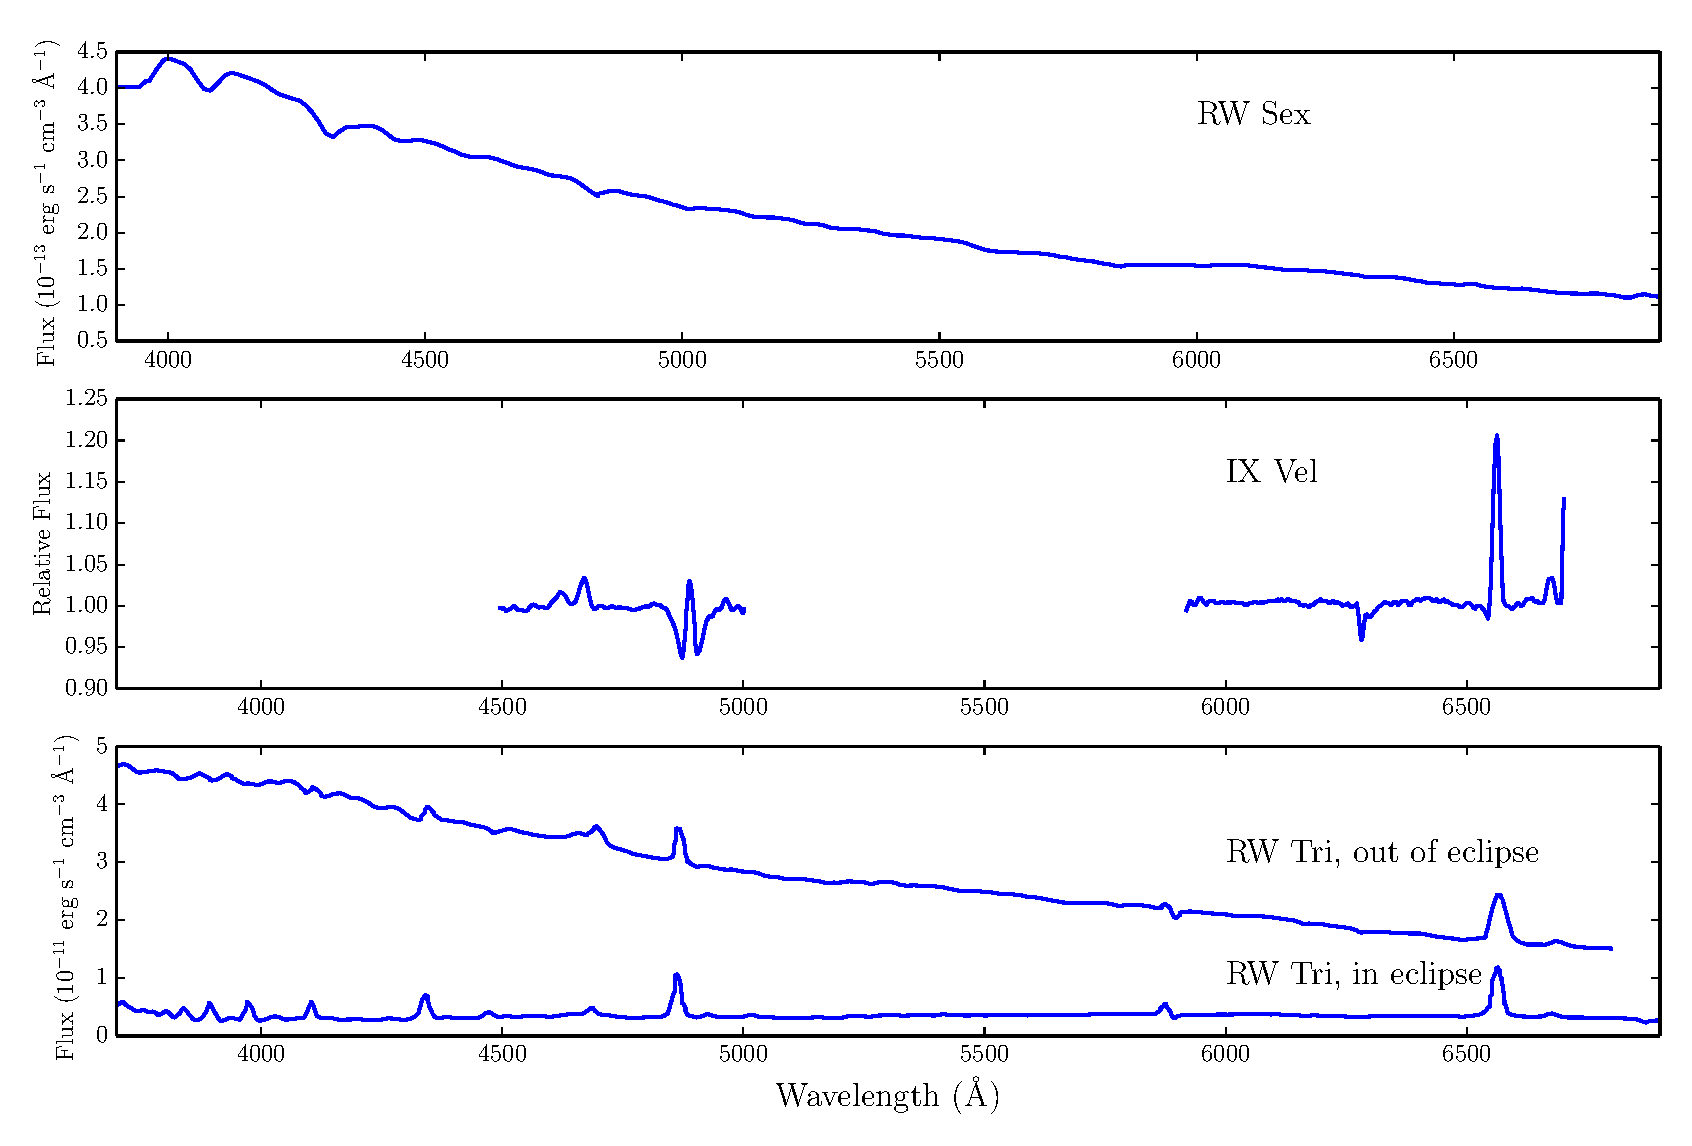
\includegraphics[width=0.8\textwidth]{figures/fig1.eps}
\caption{Optical spectra of three nova-like variables: 
RW Sex (Top; Beuermann et al. 1992),
IX Vel (Middle; Beuermann \& Thomas 1990)
and RW Tri in eclipse (Bottom; Groot et al. 2004).
The data have been digitized from the respective publications. 
These systems have inclinations of $30^\circ$, $60^\circ$ and $70^\circ$ 
respectively.
The trend of increasing Balmer line emission with inclination can be seen.
In RW Tri strong single-peaked emission in the Balmer lines is seen even
in eclipse, indicating that the lines may be formed in a spatially extensive disk wind, and there is even a suggestion
of a (potentially wind-formed) recombination continuum in the eclipsed spectrum.}
\label{novalikes}
\end{figure}

The first attempts to model disk winds in CVs applied techniques used in stellar
wind modeling to an accretion disk geometry (Mauche \& Raymond
1987; Drew 1987; Vitello \& Shlosman 1988), and showed that mass loss rates of
$\sim10\%$ of the accretion rate
were required to produce the observed line strengths.
Using spectral synthesis codes to model resonance scattering,
Shlosman \& Vitello (1993; hereafter SV93) and Knigge, Woods \& Drew (1995; hereafter KWD95)
were both successful in reproducing the observed spectra such as the P-Cygni like
profiles in C\textsc{iv}~$\lambda1549$\AA.
Long \& Knigge (2002) expanded on the above work by presenting our code, which
solved self-consistently for thermal and ionization balance in the wind
according to the methods of Mazzali \& Lucy (1993; ML93). They successfully reproduced
UV resonance lines profiles and presented a synthesized spectrum of Z Cam
that agreed well with the observed features. Noebauer et al. (2010) expanded on this
by carrying out more detailed comparisons to RW Tri and UX UMa. In addition to these 
radiative transfer calculations, some work has also been done using Hydrodynamic wind models, 
such as that by \cite{pkdh2002}, and more recently by \cite{kusterer2014} with application to
AM Canum Venaticorum stars.


Here we present work using the same Monte Carlo radiative transfer code as LK02, but incorporating additional 
`macro-atom' techniques suggested by Lucy (2002, 2003) to improve our treatment of the Hydrogen and Helium
optical lines, as well as recombination continuum emission. 
In section 2 we present the code
and provide a brief description of macro-atoms and the radiative transfer methods we employ. 
We describe the kinematics and geometry of our biconical wind model in section 3.
In section 4 we present a benchmark model, which is discussed in section 5 with particular attention 
devoted to a small-scale parameter search.
Finally, in section 6, we summarise our findings, and outline areas for future work.








%%%%%%%%%%%%%%%%%%%%%%%%%%%%%%%%%%%%%%
%
%          THE CODE, RADIATIVE TRANSFER
%
%%%%%%%%%%%%%%%%%%%%%%%%%%%%%%%%%%%%%%%

\section{Radiative Transfer}

\py is a Monte Carlo (MC) radiative transfer code which uses
the Sobolev approximation to treat line transfer. It operates 
in two distinct cycles. First, the ionization state, level populations
and temperature structure are calculated. This is done by
flying MC energy quanta through a pre-defined wind geometry and recording
the relevant estimators, before choosing  a new electron temperature 
in an attempt to balance heating and cooling in the plasma.
This process is repeated until the code converges on a 
solution. Second, the spectrum is synthesized by tracking
the energy packets through the wind and computing the 
emergent spectra at a number of user-specified viewing angles.

The code is capable of operating in a number of different
regimes, both in terms of the scale of the system, and the 
shape and characteristic energies of the illuminating spectrum. It is 
first described by LK02, who initially developed a biconical CV 
wind model to synthesize UV spectra. 
Higginbottom et al.\nocite{higginbottom2013} (2013; hereafter H13) presented a 
benchmark model for broad absorption line (BAL) QSOs.
As part of this effort, the ionization scheme was improved so that 
the code was capable of treating the power-law X-ray spectrum
exhibited by AGN.
This involved using a spectral model the mean intensity in a cell
computed from MC estimators for, instead of using a dilute blackbody
approximation. Compton processes
were also incorporated into the heating and cooling balance.
In addition, \cite{simmacro2005} modeled
Brackett and Pfund line profiles in YSOs using \textsc{Python,} which included
implementing a `macro-atom' mode in order to correctly treat the more
complex transition matrix involved in recombination. 



\subsection{Macro-atoms}

Previously, \py used a two-level atom approximation \cite[see e.g.][]{mihalas}. This approximation is 
fast, and works well as a first approximation when treating so-called `resonance lines' (such as C\textsc{iv}) 
in which the excited electron is strongly coupled to the ground state.
However, in a number of situations, for example, when a level is primarily populated from above then,
this becomes a poor representation. 
To reproduce recombination lines and lines in which the lower level is not the ground state, 
it is therefore important to use an improved line transfer technique and level population solver.

By quantising matter into `macro-atoms', and radiant and kinetic 
energy into indivisible energy packets (r- and k- packets respectively), 
Lucy (2002, 2003\nocite{lucy2002, lucy2003}; hereafter L02, L03) showed that it is possible 
to asymptotically reproduce the emissivity of a gas in statistical equilibrium 
without simplifying the treatment of line transfer. 
It allows all possible transition paths from a given level and a full non-Local 
Thermodynamic Equilibrium (NLTE) solution for the level populations based on MC estimators. 
For a full description consult L02 and L03. 

Macro-atoms have been used to model astrophysical plasmas in 
Wolf-Rayet star winds \cite{sim2004}, AGN disk winds \citep{simlong2008, tatum2012}
and Supernovae \citep{kasen2006, kerzendorfsim}.
Sim et al. (2005) used \py itself to apply this technique to
a Hydrogen-only model. We are now able to adopt a hybrid scheme. 
Any species in which have their level populations determined by
more complex interactions than resonance transitions
can be treated as full macro-atoms. The other species are treated as so-called `simple-ions',
where they still follow the indivisible packet constraint but use the two-level atom approximation.
This allows one to preserve the fast treatment of resonance lines while providing 
an improved representation of, for example, recombination, which is important when modeling features 
such as the Balmer lines and also recombination {\sl continuum} emission. 
Recombination is expected to be an important process in the optical
spectra of CVs, and they thus make a perfect application for Lucy's 
advances in MC methods.


\subsection{Ionization and Excitation}

In our hybrid ionization and excitation scheme, 
simple-ions have their ionization fractions
calculated using a modified Saha equation, and internal level populations are
calculated from LTE. For macro-atoms, we solve the equations of statistical 
equilibrium using MC estimators for the radiation field. This enables us to 
determine the ionization and excitation state of the ions in question.

\subsubsection{Macro-atoms}
% In order to correctly model lines in which the lower level is not the ground state 
% (such as H$\alpha$ \& H$\beta$), and improve the treatment of recombination,
% we treat H \& He as macro-atoms. This is because 
% the levels responsible for the line emission are populated mostly from above.
% Therefore, 
we treat H \& He as macro-atoms. 
Macro-atom NLTE level populations and ion fractions are calculated by solving 
the statistical equilbrium equations between each pair of levels. The rate
between a lower level $l$ and upper level $u$ in an atom is given by

\begin{eqnarray}
{\cal R}_{ul} &= & \beta_{lu} A_{ul} n_l + \beta_{lu} B_{ul} n_l J_{lu}^b + C_{ul} n_u n_e\label{eq:nlte_rul}\\
{\cal R}_{lu} &= & \beta_{lu} B_{lu} n_l J_{lu}^b + C_{lu} n_l n_e,
\end{eqnarray}


where $A$ and $B$ are Einstein coefficients, $C$ is the collisional rate coefficient and
$\beta_{lu}$ is the probability that a given line photon will escape the Sobolev
region. $J^b$ is the MC estimator for mean intensity at the blue wing of the line as 
recorded during the photon propagation. In the context of 
bound-free, we consider rates between the continuum state (or, in the case of ions with more than one 
bound electron, the ground state of the upper ion), $\kappa$,
and lower level $l$,

\begin{eqnarray}
{\cal R}_{\kappa l} &= & \alpha_{\kappa l} n_{\kappa} n_e \\
{\cal R}_{l \kappa} &= & n_l \int_{\nu_0}^{\infty} \frac{ 4 \pi J_{\nu} \sigma_{\nu}}{h \nu} d\nu,
\end{eqnarray}

where $\sigma_{\nu}$ is the photoioniziation cross section, $\alpha_{\kappa l}$ is the recombination
coefficient to level $l$ and $J_{\nu}$ is the mean intensity.
This treatment means that radiative and collisional rates to and from all 
levels are considered when calculating both the ionization state, and the level populations, 
although we neglect photoionization to excited levels of the upper ion. 
The \cite{vanregemorter} approximation is used for collisional transitions,
and thus we assume collisions between radiatively forbidden collisions are
negligible, a reasonable approximation in the regime where levels are mainly populated
by recombination. 
%{2002A&A...384..725L}.  source for beta sobolevs
%$\beta_{lu}=\frac{1}{\tau_{lu}}[1-\exp(-\tau_{lu})]$

\subsubsection{Simple-ions}

C, O, N, Ne, Na, Mg, Al, Si, S, Ar, Ca \& Fe are all included as simple-ions. 
The two-level atom is a first order approximation here, which is appropriate 
when treating resonance lines in which the lower level is at or close to the 
ground state. 
For these elements, we follow LK02 in using the ionization scheme presented by Mazzali \& Lucy (1993). 
Specifically, we use the formula
\begin{equation}
\frac{n_{j+1} n_e}{n_j} = W [\xi + W(1-\xi)]
\left(\frac{T_e}{T_R}\right)^{1/2}
\left(\frac{n_{j+1}n_e}{n_j}\right)^*_{T_R} \label{ionization}
\end{equation}
to solve for the relative ionization fractions. In this equation, the `starred' term on 
the right represents the Saha abundances, in accordance with the notation of Mihalas (1982). 
$W$ is an effective dilution factor, $\xi$ is the
fraction of recombinations going directly to the ground state, and
$T_R$ and $T_e$ are the radiation and electron temperature
respectively. LK02 provide a full description of our implementation.

The reason for using this scheme 
is twofold; First, unlike in H13, the SED can be approximated well by a dilute blackbody due to the 
absence of a power-law X-ray source, and therefore the above modification to the Saha equation
is appropriate; Second, this provides continuity from LK02 and allows us to do a like-for-like comparison,
which is especially useful in assessing the improvement in Hydrogen line emission, and any changes
that might occur in the ionization stages of the resonance line species such as CIV. 
Excitation is then calculated from LTE approximations. 
%This is because the 
% level populations are only important in working out the resonance scattering 
% opacity through the wind when modeling resonance lines.



\subsection{Atomic Data}
Atomic data is obtained from the same sources described in LK02 and updated in H13. 
The additional level and line information required to treat He as macro atom was 
obtained from \textsc{Topbase} \citep{topbase2005}. We treat H as a 20-level atom as in S05, where 
each level is defined by the principal quantum number n, which is appropriate due to
the degeneracy of each level in the H atom. He~\textsc{II} is treated in much the same way,
with 10 levels, but He~\textsc{I} has larger energy differentials between different l subshells
and triplet and singlet states. Thus, we still include levels up to $n=10$ but explicitly 
treat the $l$ and $s$ sub-orbitals as distinct levels instead of assuming they are perfectly `l-mixed',
which also allows the model to produce singlet and 
triplet lines, as seen in optical CV spectra.



\subsection{Code Validation and Testing}

\py has previously been tested against a number of radiative transfer and
photoionization codes. Comparisons of ionization balance with \cld \citep{cloudy2013} 
can be found in LK02 and H13 showing excellent agreement. We have also conducted comparisons
of ionization and spectral synthesis with the supernova code \textsc{Tardis.} \tar is described by
\cite{kerzendorfsim}, and the spectral comparisons can be found therein.
In addition to these code validation efforts, we have also conducted tests of
the macro atom scheme in \py to verify that it does indeed solve for level populations correctly
and produces the correct level emissivities. We have been able to show good agreement with 
Case A and Case B calculations by \cite{seaton1959}, and have tested our level
population solver against \textsc{Tardis.}

%% include figure here

% The left panel of figure~\ref{seaton} shows a comparison
% between our level emissivities for the Balmer series compared with analytic calculations
% by \cite{seaton1959}, showing good agreement in both the Case A and Case B limits 
% (see Osterbrock 1989 for a discussion of these two commonly used approximations\nocite{osterbrock}).
% The right panel of figure~\ref{seaton} shows a comparison of Helium I level populations (the most
% complex ion we currently treat as a macro-atom) between \py~and \tar~models. Considering the 
% two codes use different atomic data and \textsc{Tardis,} unlike \textsc{Python,} currently has a complete treatment of
% collisions between radiatively forbidden transitions, the factor of $<2$ agreement is 
% encouraging. 


%%%%%%%%%%%%%%%%%%%%%%%%%%%%%%%%%%%%%%
%
%          THE MODEL
%
%%%%%%%%%%%%%%%%%%%%%%%%%%%%%%%%%%%%%%%

\section{A Biconical Wind CV Model}

Here we describe some of the features of our biconical wind model. Our aim here is not
to provide a `best fit' model to the data, but rather to use as a starting point
the types of models which have already been successful in explaining UV spectra of CVs,
and examine their effect on the optical features when the treatment of line transfer
is improved.

\subsection{Description of Model: Geometry and Kinematics}

Our model follows the prescription outlined by Schlosman \& Vitello (1993; SV93). A schematic is shown
in figure~\ref{cartoon}. A smooth, biconical
disk wind rises from the accretion disk between radii $r_{min}$ and $r_{max}$. The covering fraction of the wind is 
controlled by the opening angles of the wind, $\theta_{min}$ and $\theta_{max}$, and the launch angle of
the other streamlines is given by

\begin{equation}
\theta(r_0) = \theta_{min} + (\theta_{max} - \theta_{min}) \left(\frac{r_0 - r_{min}}{r_{max} - r_{min}} \right)^{\gamma},
\label{theta}
\end{equation}

where $r_0$ is the launch radius of the streamline.
As in LK02, we follow SV93's power law
velocity profile. The poloidal velocity, $v_l$, in our model is given by

\begin{equation}
v_l=v_0+\left[v_{\infty}(r_0)-v_0\right]\frac{\left(l/R_v\right)^{\alpha}}{\left(l/R_v\right)^{\alpha}+1},
\label{v_law}
\end{equation}

where $l$ is distance measured along a  streamline. $v_{\infty}$, the 
terminal velocity, is set to a fixed multiple of the escape velocity at the bottom
of a streamline, and $v_0$ is a constant launch velocity (set to $6$~km~s$^{-1}$).
Once the wind is launched, it accelerates with a characteristic acceleration
length $R_v$, and $\alpha$ is an exponent which controls how quickly the 
wind accelerates. Larger values of $\alpha$ cause the main region of 
acceleration to occur close to $R_v$, whereas smaller values will lead
to a fast acceleration close to the disk (see figure~\ref{acc_law}).
SV93 chose this velocity law so as to give a 
velocity gradient that varied continuously along a streamline, as well
as producing line profiles with realistic velocity spreads.
In addition to these motivations, adopting a consistent velocity law 
allows for direct comparison with models which have already been successful in 
simulating UV resonance line profiles, such as those presented by LK02 and SV93.  


\begin{figure}
\centering
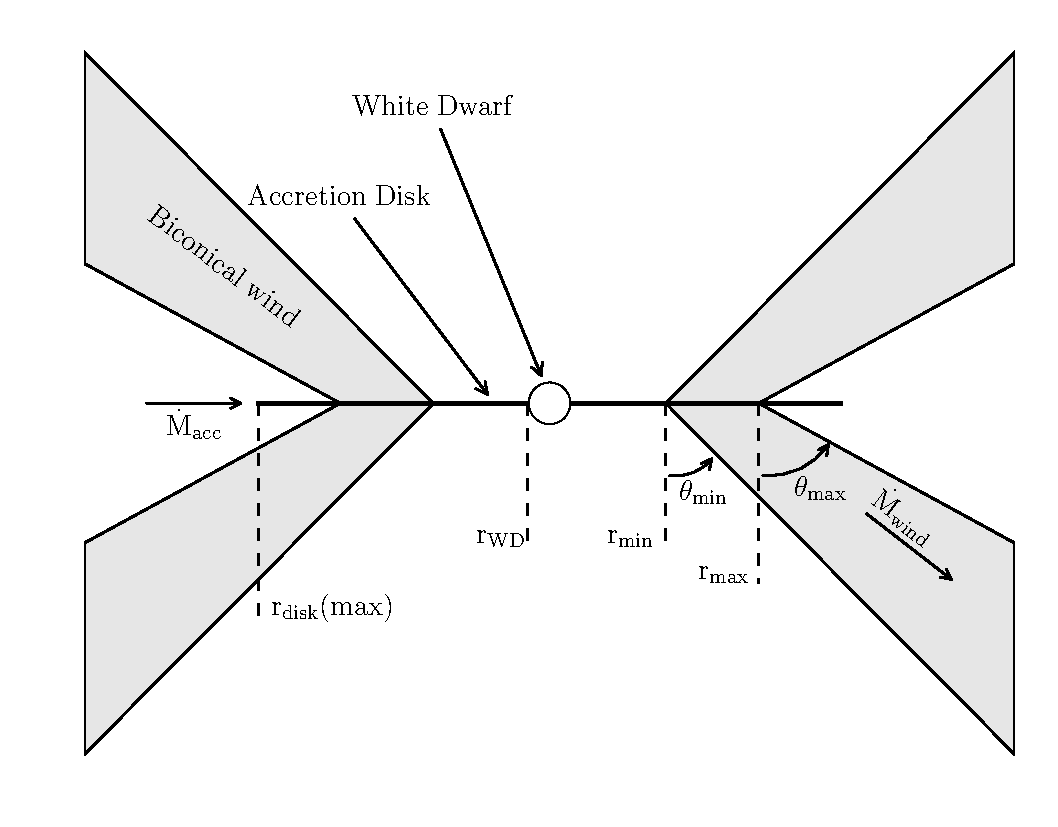
\includegraphics[width=0.5\textwidth]{figures/fig2_cartoon.eps}
\caption{Cartoon illustrating the geometry and kinematics of the benchmark CV wind model.}
\label{cartoon}
\end{figure}


\begin{figure}
\centering
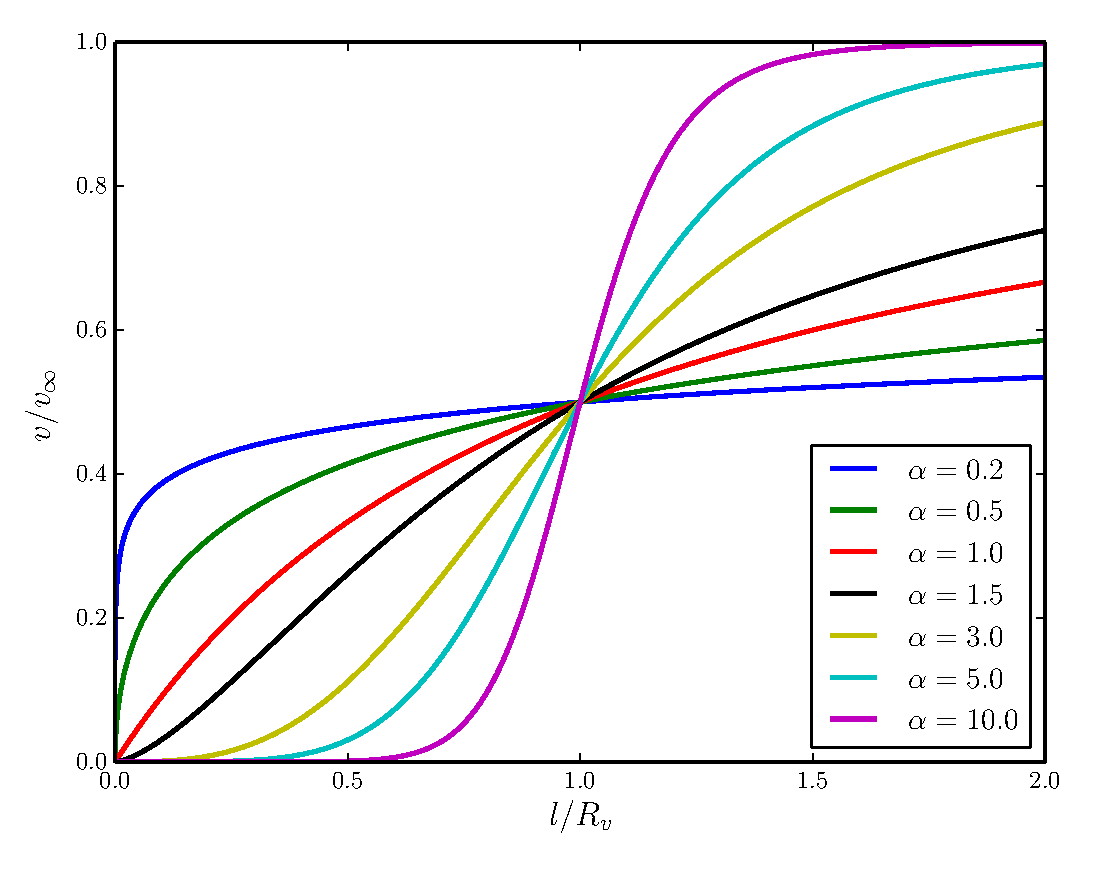
\includegraphics[width=0.45\textwidth]{figures/acc_law.eps}
\caption{
The velocity law in our model for various values of
the acceleration exponent.
}
\label{acc_law}
\end{figure}


\begin{table}
\centering
\begin{tabular}{p{3cm}p{4cm}}
Model A \\
\hline Free Parameters 	&	 Value \\ 
\hline \hline 
$M_{WD}$ 	 &	 $0.8 M_{\odot}$ \\ 
$\dot{M}_{acc}$ 	 &	 $10^{-9}~M_{\odot}yr^{-1}$\\ 
$\dot{M}_{wind}$  &	$10^{-8}~M_{\odot}yr^{-1}$\\ 
$r_{min}$ 	&	 $4 R_{WD}$\\ 
$r_{max}$ 	&	 $12 R_{WD}$ \\ 
$\theta_{min}$ 	&	 $20.0^{\circ}$ \\ 
$\theta_{max}$ 	&	 $65.0^{\circ}$ \\ 
$\gamma$ 	&	 $1$ \\ 
$v_{\infty}$ 	&	 $3v_{esc}$ \\ 
$R_v$ 	        &	 $7\times10^{10}$cm \\ 
$\alpha$ 	&	 $1.5$ \\
\end{tabular}
\centering
\caption{
Wind geometry parameters used in the benchmark CV model.}
\label{wind_param}
\end{table}


The principle of mass conservation means that the velocity law also 
controls the density, $\rho$, of the wind, which can be expressed in terms
of radial and vertical position $(r,z)$ as 

\begin{equation}
\rho(r,z) = \frac{r}{r_0} \frac{dr}{dr_0} \frac{\phi(r_0)}{v_z(r,z)},
\label{density}
\end{equation}

where $\phi$ here is the mass loss rate per unit area at $r_0$
and $v_z$ is the vertical velocity component. In this model, we
adopt a uniform value for $\phi$. 



\subsection{Photon Sources}

MC quanta originate from an accretion disk and a central WD in our model. It is also possible to include
a boundary layer with user-defined temperature and emitting area. Emission from the wind is dealt with
by reprocessing of the indivisible energy packets originally produced in the disk or central WD.

\subsubsection{Disk Treatment}

\py has has some flexibility when treating the accretion disk as a source of photons. 
The disk is broken down into annuli 
such that each annulus contributes an equal amount to the bolometric luminosity. 
We adopt the temperature profile of a standard \cite{shakurasunyaev1973} $\alpha$-disk.
%shown in figure 1.
An annulus can then
be treated either as a blackbody with the corresponding effective temperature or as a stellar atmosphere model
with the appropriate surface gravity and effective temperature. 
Both of these methods have limitations. It is known
from studies of CV accretion disks that they exhibit absorption cores 
formed in an optically thick disk atmosphere.
This can impact the overall spectrum even if a wind is present 
\citep[see e.g.][]{dhillon1996}.
However, the stellar atmosphere models
have had difficulties reproducing the required spectral shape \citep{wade1988}, 
and there are inconsistencies when using a 
stellar atmosphere beneath a dense
wind region that itself goes some way to simulating the disk atmosphere. 
In addition, \cite{linnell2010} found that deviations from the predicted 
$T\propto r^{-3/4}$ temperature profile are required to fit the data
in certain cases. 

We hope that future simulations, coupled with a comparison to data, will 
actually address some of these problems, particularly since
the filtering effect of the wind may cause noteiceable effects
on the colour of the emergent spectrum \citep{hassall}. 
Here we use a blackbody illuminating spectrum
for the ionization cycles (see figure~\ref{sed}) and to compute our MC estimators.
During the spectral synthesis stage of the simulation we use stellar atmosphere models.
This is partly because they provide the most pessimistic prediction in terms of whether recombination emission in the 
wind can fill in the Balmer jump, due to the strong absorption beyond the Balmer edge.
For low temperatures, we use stellar atmospheres computed 
by Kurucz (reference), and for $T>50,000$~K we use models computed with 
\textsc{TLUSTY} \citep{tlusty}. The input spectra are created from these model
atmospheres using \textsc{Synspec}\footnote{http://nova.astro.umd.edu/Synspec43/synspec.html}.
%The temperature profile of our disk,
%with $\dot{M}_{acc} = 10^{-8}~M_{\odot}yr^{-1}$ can be seen in figure~\ref{t_profile}.

\begin{figure}
\centering
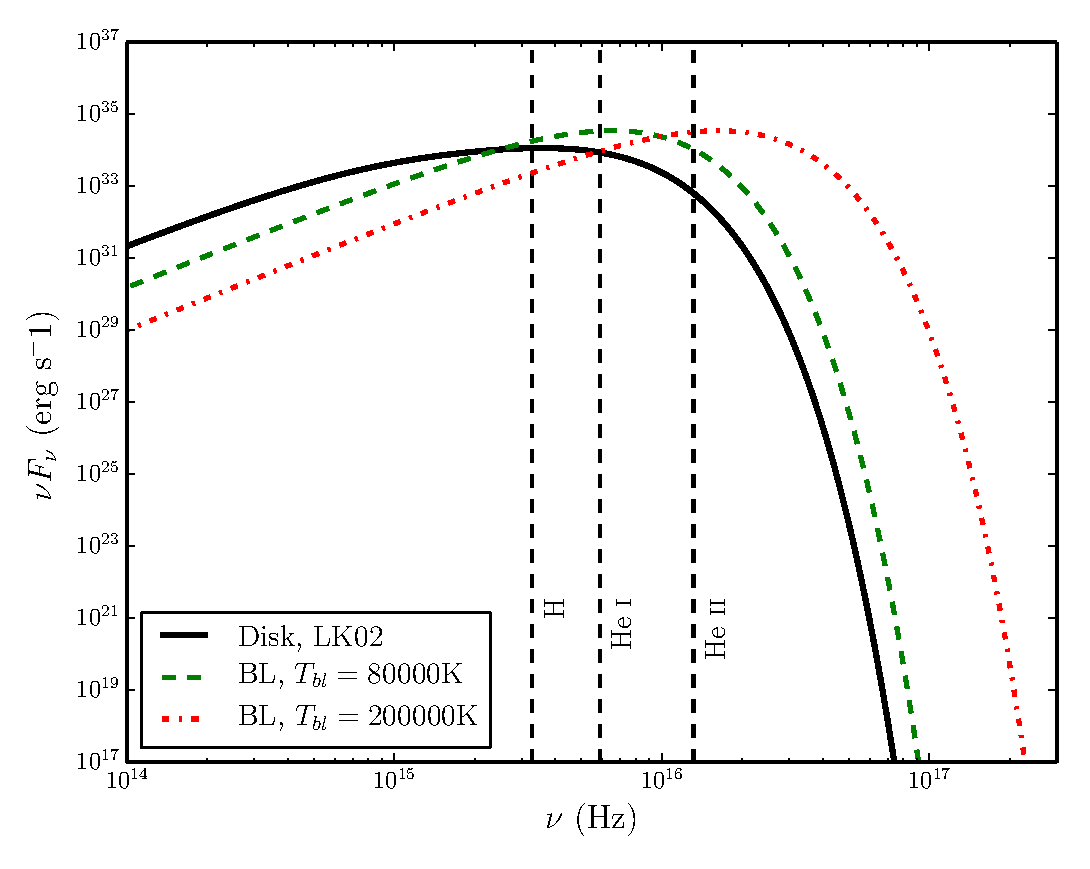
\includegraphics[width=0.45\textwidth]{figures/sed_figure.eps}
\caption{
The spectral energy distribution of the blackbody accretion
disk used in the ionization calculation (thick black line), 
with two boundary layer spectra also plotted.
The positions of the Hydrogen and Helium ionization edges 
are marked with dashed vertical lines.
%The effective temperature of the accretion disk
%in our model, as a function of radius.
}
\label{sed}
\end{figure}



\subsubsection{Boundary Layer}
The existence of a boundary layer in CVs arises naturally from the boundary condition
of the \cite{shakurasunyaev1973} model, since the material at the inner disk
edge must lose angular momentum in order to be deposited on
the surface of the compact object \cite[see e.g.][]{lyndenbell1974}.
Boundary layers are a possible source of
high energy photons which may be responsible for the photoionization of 
He~\textsc{ii}. 
\cite{pringlesavonije1979} predict temperatures of 
$200,000-500,000{\rm K}$ for the boundary layer,
but a number of studies have found difficulties
in producing the required ionization state of the wind
with such a hot, luminous boundary layer 
\citep[see e.g.][]{maucheraymond1987, drewverbunt1985}.
\cite{hoare1991}
use the Zanstra method to find boundary layer temperatures of
$\sim80,000{\rm K}$


It is possible to include a boundary layer in our model which emits 
as a blackbody with the effective temperature

\begin{equation}
T_{bl} = \left[ \frac{L_{acc}}{8 \pi R_* H \sigma} ( 1 - \omega_*/\omega_k)^2 \right]^{1/4},
\label{bl}
\end{equation}

where $L_{acc}$ is the accretion luminosity, $R_*$ is the WD radius, $H$ is the boundary layer height
above the disk plane
and $\omega_*$ and $\omega_k$ are the angular velocities at the WD surface and inner disk edge respectively
\citep{fkrbook}. Note that we assume a cylindrical geometry such that the effective emitting
area is $4 \pi R_* H$. 
In the benchmark model, we follow LK02 in setting the boundary layer
luminosity to zero, and then investigate the effect
of boundary layers with temperatures of $80,000{\rm K}$ and $200,000{\rm K}$ 
on the ionization state of the wind and resulting
spectrum. See section 5 for a discussion.

%Whether we include one, why why not, referring to He II and ionization.

%%%%%%%%%%%%%%%%%%%%%%%%%%%%%%%%%%%%%%
%
%          RESULTS
%
%%%%%%%%%%%%%%%%%%%%%%%%%%%%%%%%%%%%%%%

\section{Results \& Analysis from a Benchmark Model}

The results in this section were obtained using the geometry described
in section 3. The kinematics and mass loss rate of the wind are identical
to LK02. Photon sources are identical, except that when synthesizing the
spectrum we treat the accretion disk 
as an ensemble of Kurucz and TLUSTY stellar atmosphere models to better 
interpret the behaviour of the Balmer jump. The aim here is to 
take a successful UV wind model, and examine it's effect 
when one utilises the better treatment of lines provided
by the macro-atom scheme.

\subsection{Synthetic Spectra}

\begin{figure} %fullpage
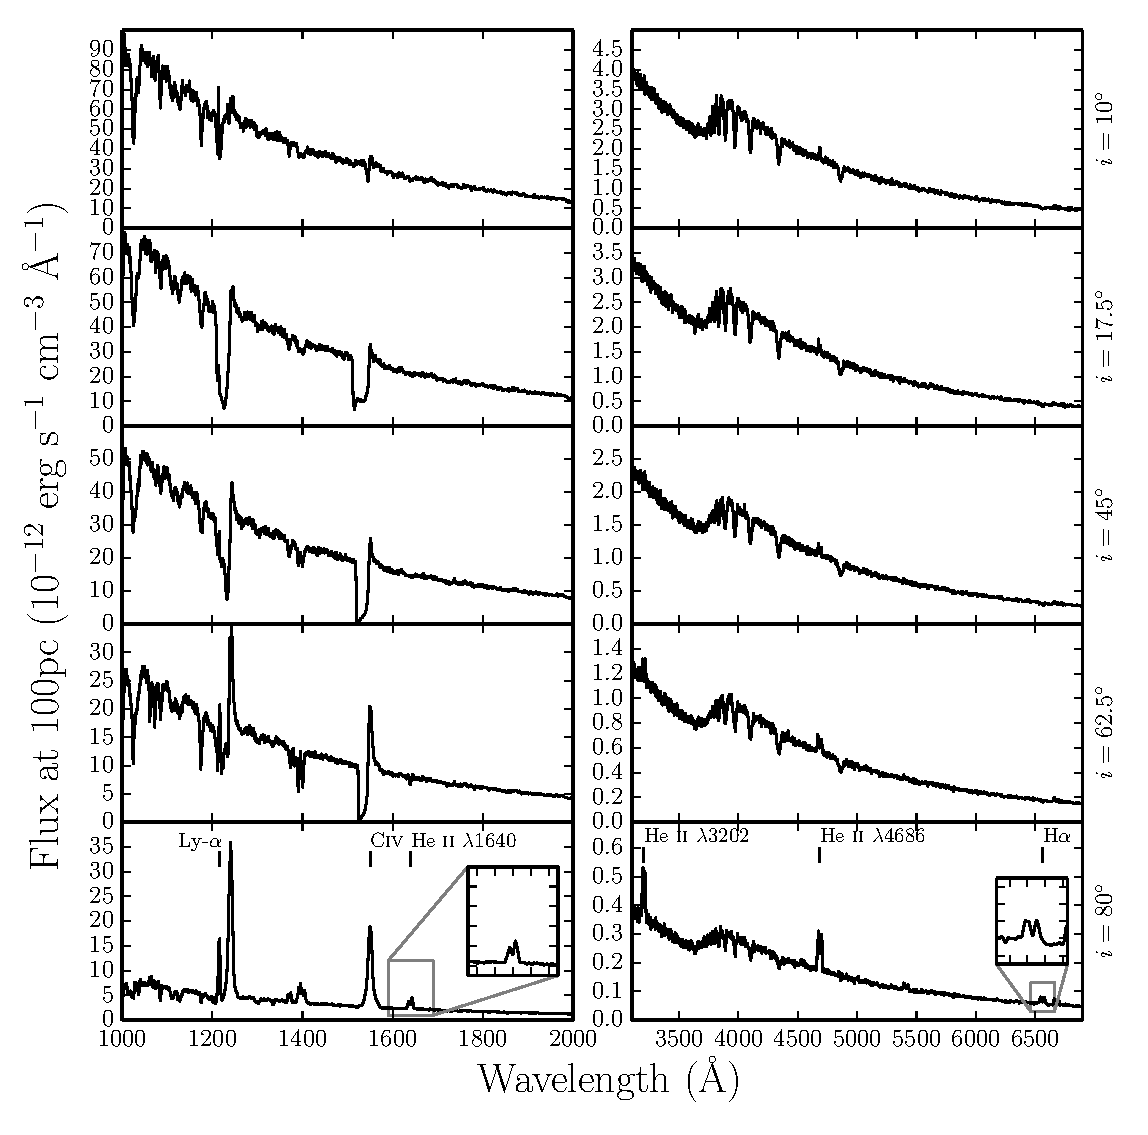
\includegraphics[width=\textwidth]{figures/fig5_uv_opt.eps}
\caption{
UV (left) and Optical synthetic spectra for model B computed at
sightlines of 10,27.5, 45, 62.5 and 80 degrees.	
The inset plots show zoomed-in line profiles for 
\heiiuv and \ha. Double-peaked line emission can be seen in 
\heiiuv, \heiiopt, \ha and some He I lines, but the 
line emission is not always sufficient to overcome the absorption
cores from the stellar atmosphere models.
}
\label{spec}
\end{figure} %fullpage\

Figure~\ref{spec} shows optical synthetic spectra for the benchmark 
model for 5 different sightlines. The first thing to note is that the 
model produces some lines which are strong enough to overcome
the absorption cores lines from the disk. These lines are generally double peaked, 
implying they were formed near the base of the wind where rotational velocity
can still dominate over the slowly increasing poloidal velocity. A Balmer 
jump is present at all inclinations. This is present
in the stellar atmosphere models used to model the disk,
and is not a result of photoabsorption through the wind.
%%%% SAY BALMER JUMP CASUED BY SAs

In fact, the wind has a Balmer jump in emission, but it is not prominent enough
to overcome the intrinsic absorption in the illuminating spectrum. 
Figure~\ref{cont} shows the total escaping spectrum, integrated
over all viewing angles, with the contribution from the disk and wind
also plotted. It shows that the lines are produced in the wind,
and also that the wind is producing a Balmer recombination
continuum, but one which is not yet sufficient to mask the absorption 
intrinsic to the disk SED. This offers a tantalising hint
that modest changes to the kinematics of the wind
may be sufficient to boost the continuum emission of the wind.
Furthermore, it confirms our suspicions that the improved
radiative transfer would cause enhanced recombination emission,
suggesting that, where possible, up to date treatments of
NLTE line transfer should be used in codes such as this.


The prominent P-Cygni profiles in e.g., C\textsc{iv} are still seen
in the UV spectra (see figure~\ref{spec}). In addition, the wind 
now contributes significant Lyman-$\alpha$ and
He~\textsc{ii}~$\lambda1640{\rm \AA}$  emission. 
We note that the ionization state of the wind 
is such that recombination to He~\textsc{ii} is significant, even
without a boundary layer source of higher energy photons.

\begin{figure} 
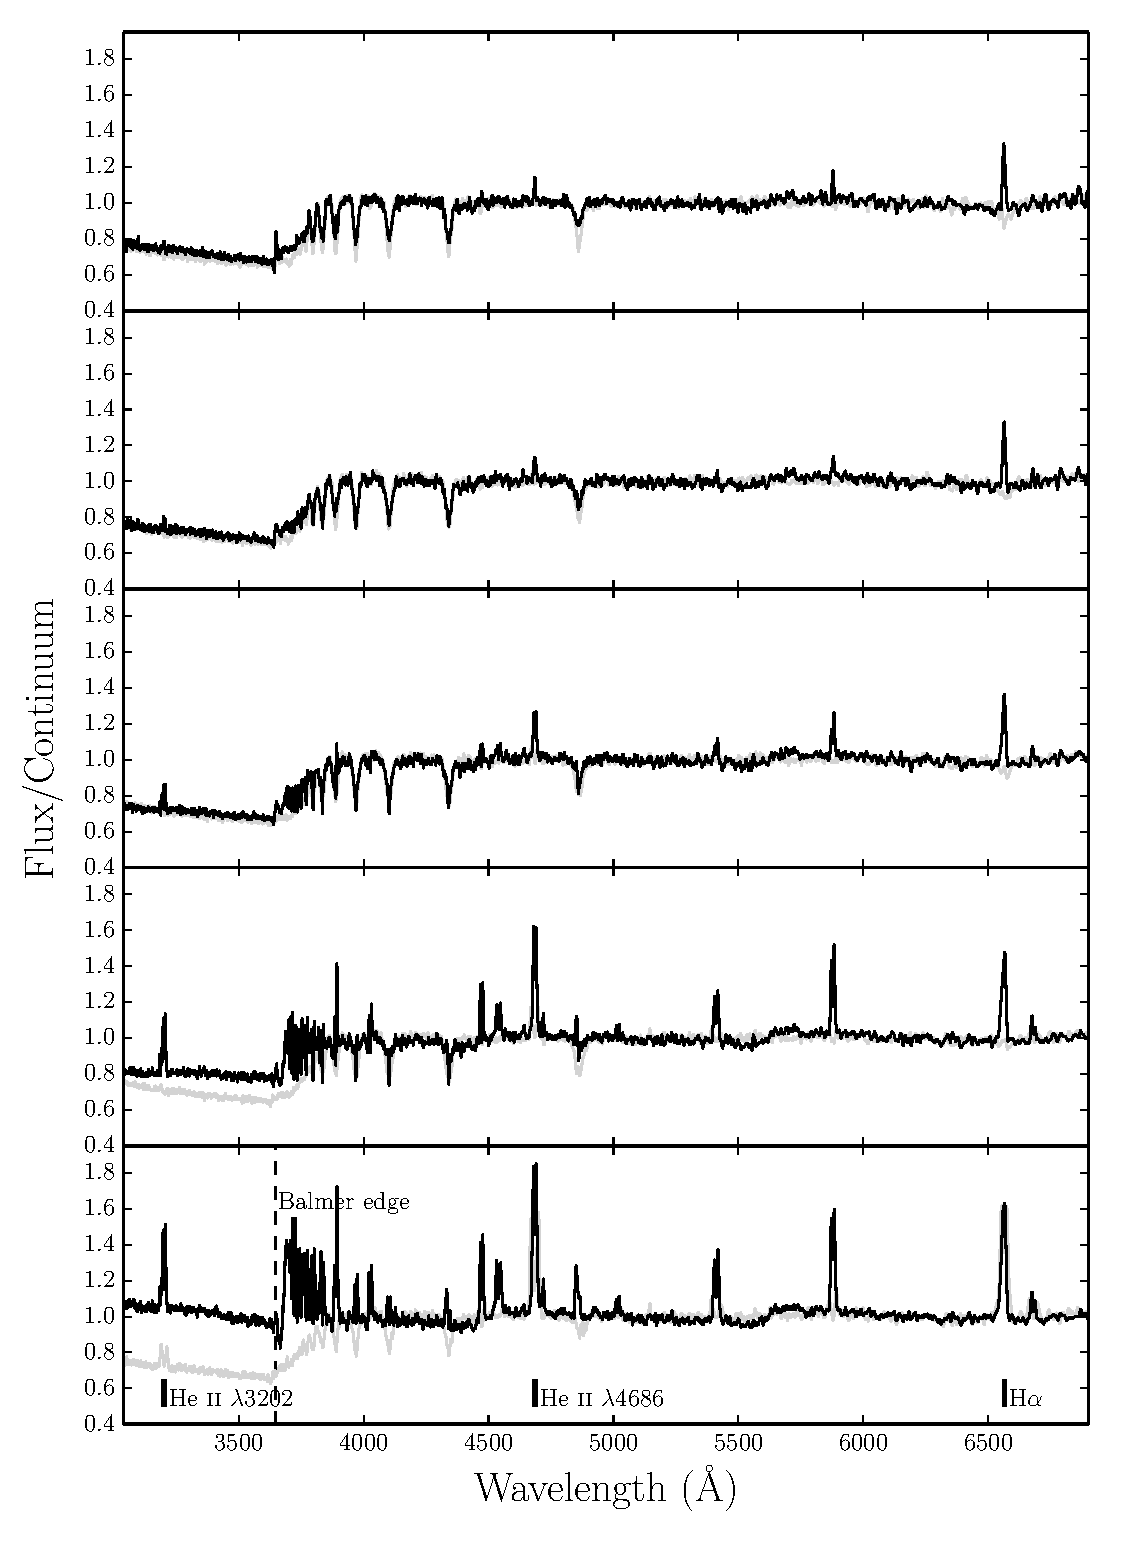
\includegraphics[width=0.45\textwidth]{figures/fig6_opt_cont.eps}
\caption{Synthetic optical spectra computed for sightlines of 22.5, 25, 62.5 and 80 degrees.}
\label{spec_continuum}
\end{figure} 



Clearly, this particular model cannot explain all
the features seen in the optical spectra of Nova-like variables. However,
the wind has a clear effect on the spectral features, and cannot be ignored as 
a both source of line and continuum emission and as a reprocessing `filter'
of the underlying disk spectral energy distribution (SED).



\begin{figure} 
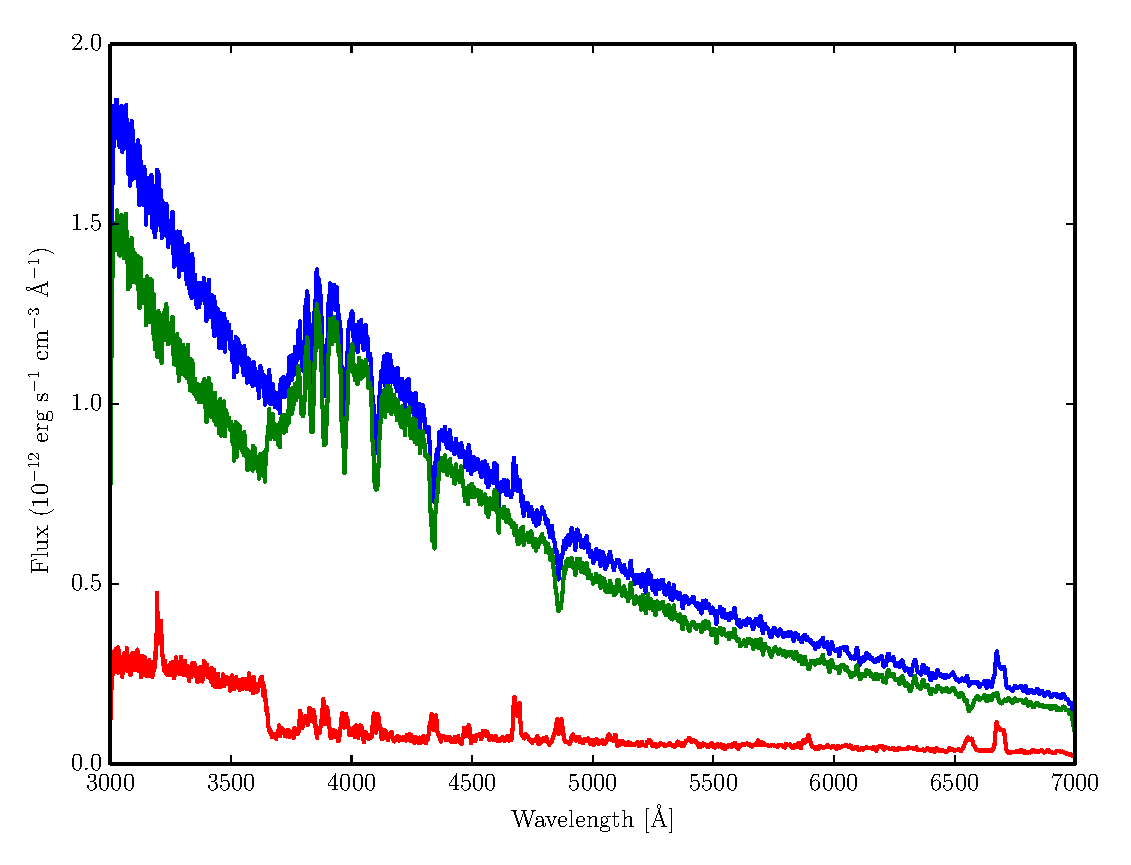
\includegraphics[width=0.5\textwidth]{figures/fig4.eps}
\caption{Total packet-binned spectra across all viewing angles. The top panel shows the total 
integrated escaping spectrum, while the other panels show the contributions from photons that originate
in the disk and wind respectively. Recombination continuum emission blueward of the Balmer 
edge is already prominent relative to other wind continuum processes, but is not sufficient
to fill in the Balmer jump in this specific model}
\label{cont}
\end{figure} 

\subsection{Ionization and Temperature Structure}

In addition to producing synthetic spectra, we are also able to 
analyse the physical properties of the outflow.
Figure~\ref{wind} shows various physical properties
of the wind geometry. The ionization structure of the wind
is very similar to the original LK02 model, as one might expect.
He is mostly ionized throughout the wind except for a small region near
the disk which is shielded from the photons produced by the hot inner disk.

C\textsc{iv} is the dominant Carbon ion throughout the wind, allowing
for an absorbing column which covers a large range of velocitieis, and is thus
sufficient to produce the required broad, deep and blue-shifted absorption lines
we expect to see in a large fraction of Nova-likes.



\begin{figure} %fullpage
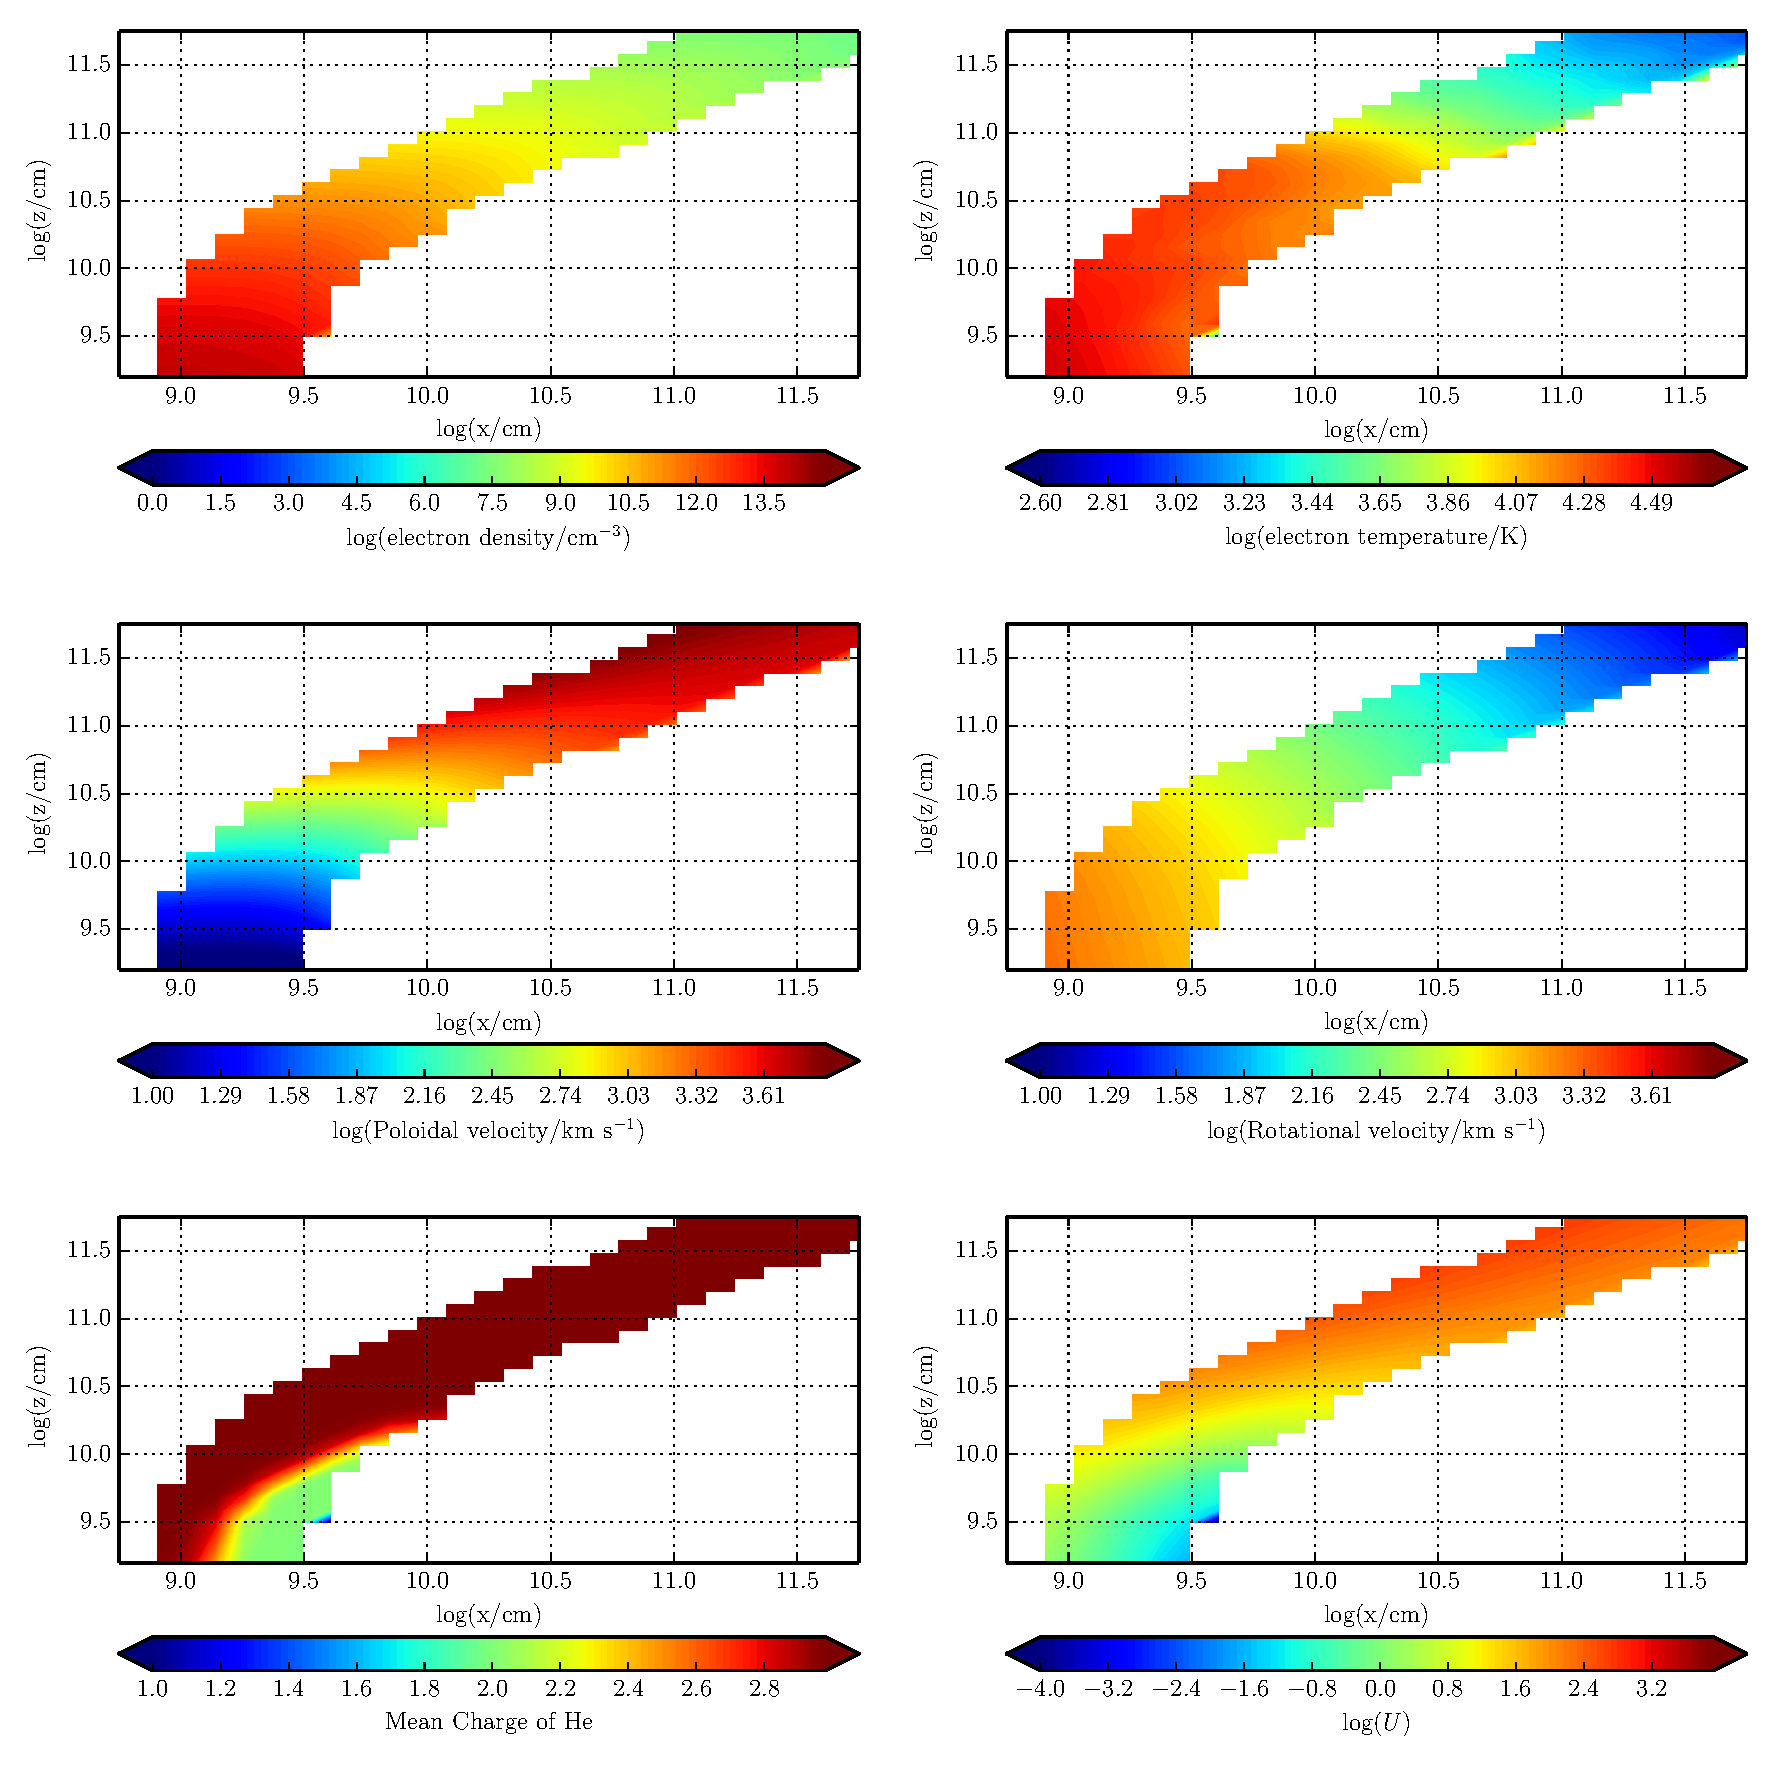
\includegraphics[width=\textwidth]{figures/fig5.eps}
\caption{Various properties of the wind.}
\label{wind}
\end{figure} %fullpage



%%%%%%%%%%%%%%%%%%%%%%%%%%%%%%%%%%%%%%
%
%          DISCUSSION
%
%%%%%%%%%%%%%%%%%%%%%%%%%%%%%%%%%%%%%%%

\section{Discussion of Results}

The benchmark model presented above shows that a wind with the properties
of Model A, a model that successfully reproduces the UV spectral features,
would leave a clear imprint on the optical spectrum. It is important
to understand how changing the kinematics of the wind impacts this
effect. We can therefore examine the evolution
of the spectrum with a few key parameters. In particular, this
will help shed light on the predictions of, e.g., Murray \& Chiang (1996)
and Knigge et al. (1998) regarding the single peaked H$\alpha$ emission
and absence of a pronounced Balmer absorption edge respectively.

\subsection{Exploring Parameter Space}

The amount of line and recombination continuum
emission produced by given ion, $i$, in a plasma of volume $V$
depends on the emission measure, $EM$, defined as

\begin{equation}
EM=\int^V_0 n_e n_i \,dV,
\end{equation}

where $n_i$ is the number density of the ion in question. 
The emission reaching an observer 
also depends on the optical depth along 
the line of sight, which can also significantly affect line profile shapes.
Therefore, any quantity which controls the density profile of the wind
will have a profound impact on both the 
amount of emission and the shape of the escaping line profiles.

As described in section 3, we can alter the density in the wind by 
adjusting the velocity law. We have therefore conducted a limited parameter 
sweep, exploring the effect of changing $R_v$, $\alpha$ and $\dot{M}_W$.


\subsection{The Balmer Lines}

\begin{figure} %fullpage
\mbox{
\subfigure{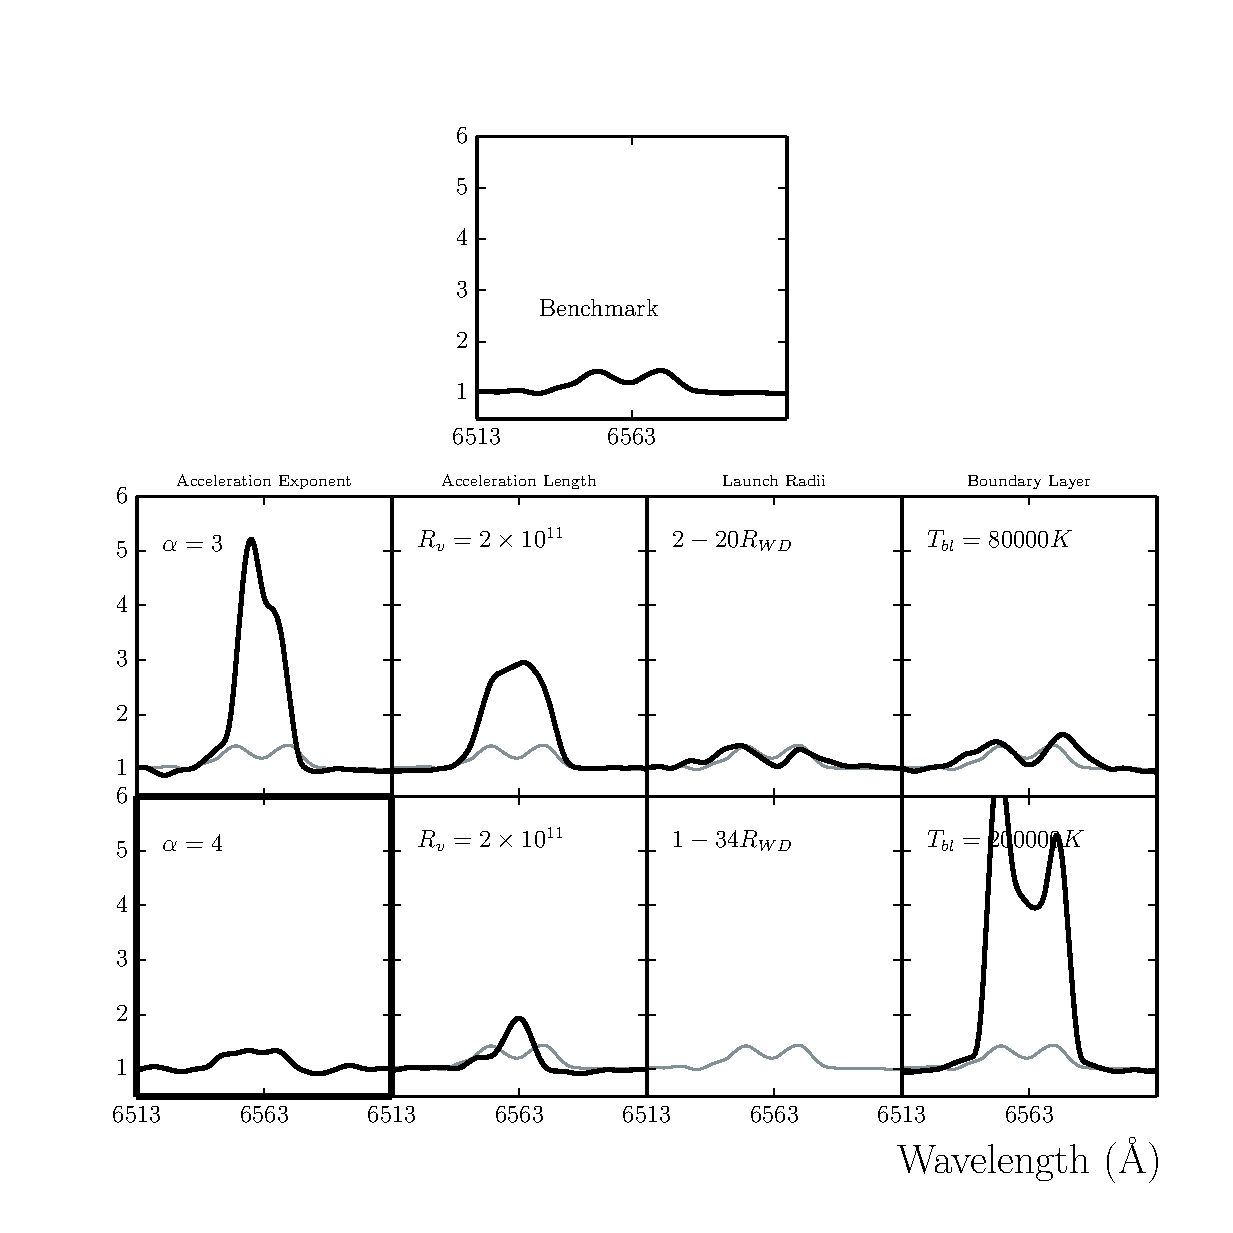
\includegraphics[width=0.5\textwidth]{figures/grid_alpha.eps}}
\quad
\subfigure{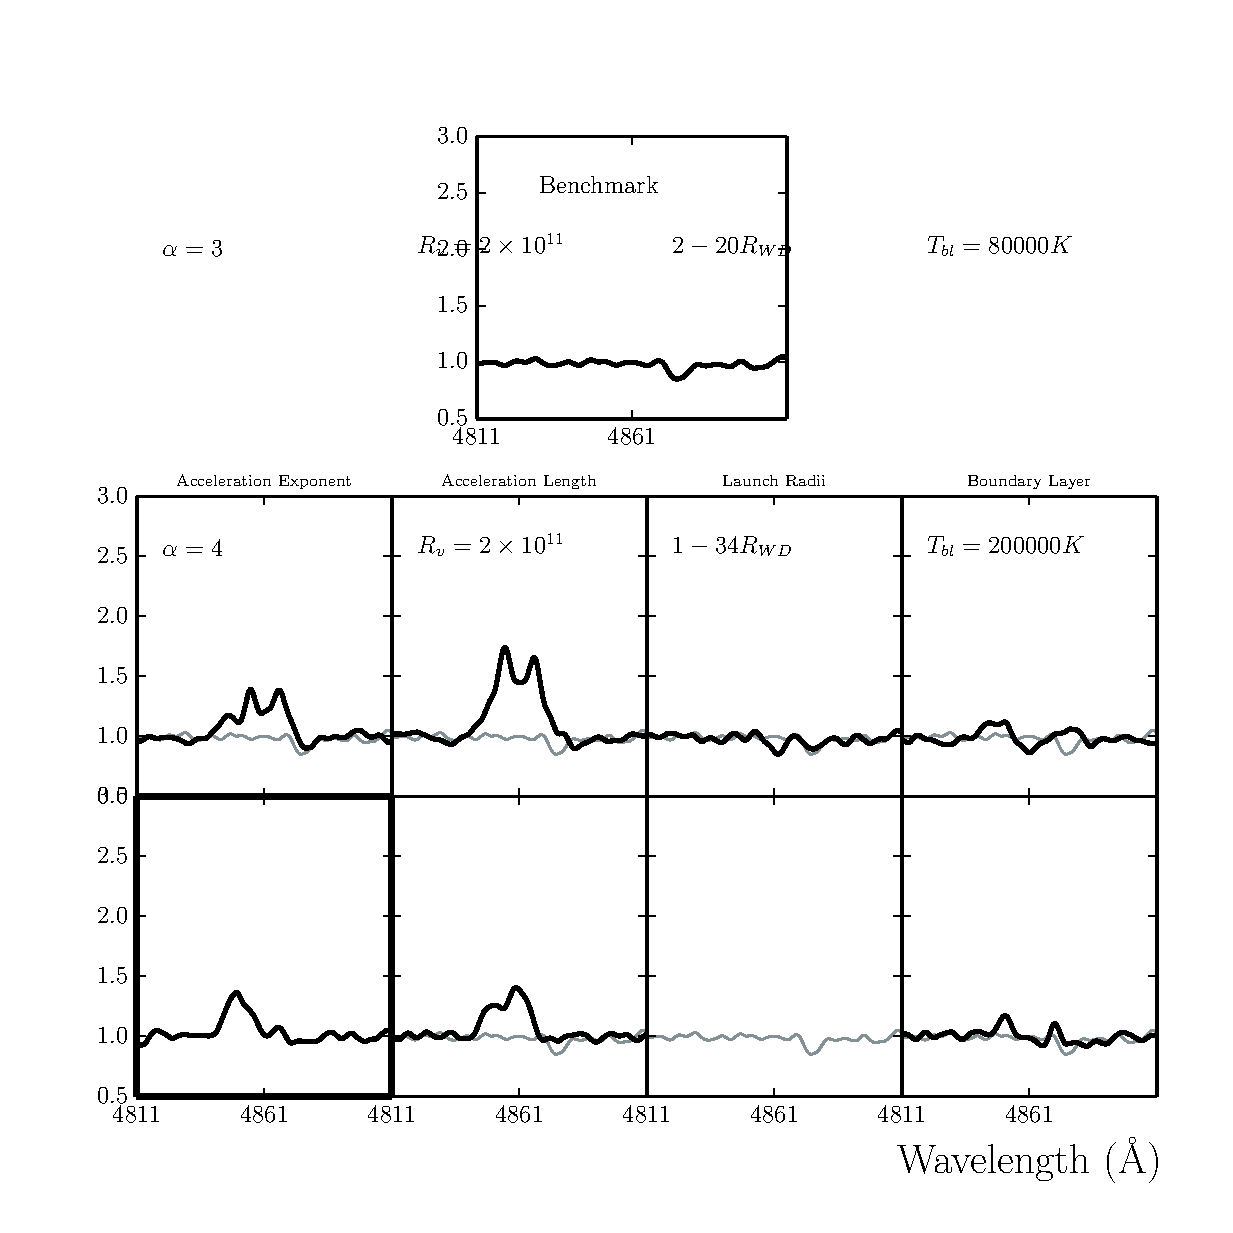
\includegraphics[width=0.5\textwidth]{figures/grid_beta.eps}}   
}
\caption{
% How the H$\alpha$ and H$\beta$ lines in our model change with the kinematic properties
% of the wind. The three separate panels show three different values of $\dot{M}_W$, 
% while $\alpha$ and $R_v$ are all gradually increased from top to bottom and left to right respectively.
% Larger values of these quantities increase the density at the base of the wind. There is a clear transition
% from double peaked to single peaked behaviour, and at the highest densities the wind
% essentially becomes neutral as the optically thick regions self-shield the wind from photoionizing radiation.
\bf{Each of these figures will highlight the next gen model in bold.
and contain a grid like the above showing a pair of spectral features in
the left and right panels. The grey shaded line will show the benchmark model
for easy comparison.  
The most promising parameters at the moment are acceleration exponent and launch radii.}
}
\label{halpha}
\end{figure} %fullpage

Figure~\ref{halpha} shows how the H$\alpha$ line changes with the kinematics 
of the wind at an inclination of $80^\circ$. For models with lower densities, the
line is double peaked, but we see a transition to a single peaked line when 
a high enough density is reach such that the line becomes optically thick.
This reproduces the behaviour predicted by \cite{MC96}, who suggested that
the poloidal velocity gradient in the wind can be larger than the gradient of 
the Keplerian velocity. This gradient can therefore modify the line profile shape
but requires the line to be optically thick.

\subsection{The Balmer Jump}



\label{balmerjump}
\begin{itemize}
\item that we are able to fill in the Balmer jump with the recombination continuum from the wind
if the EM is high enough
\item How this changes with inclination
\item Comparison to literature
\item Discussion of disk atmosphere treatment and its effect.
\end{itemize}

\begin{figure} %fullpage
\mbox{
\subfigure{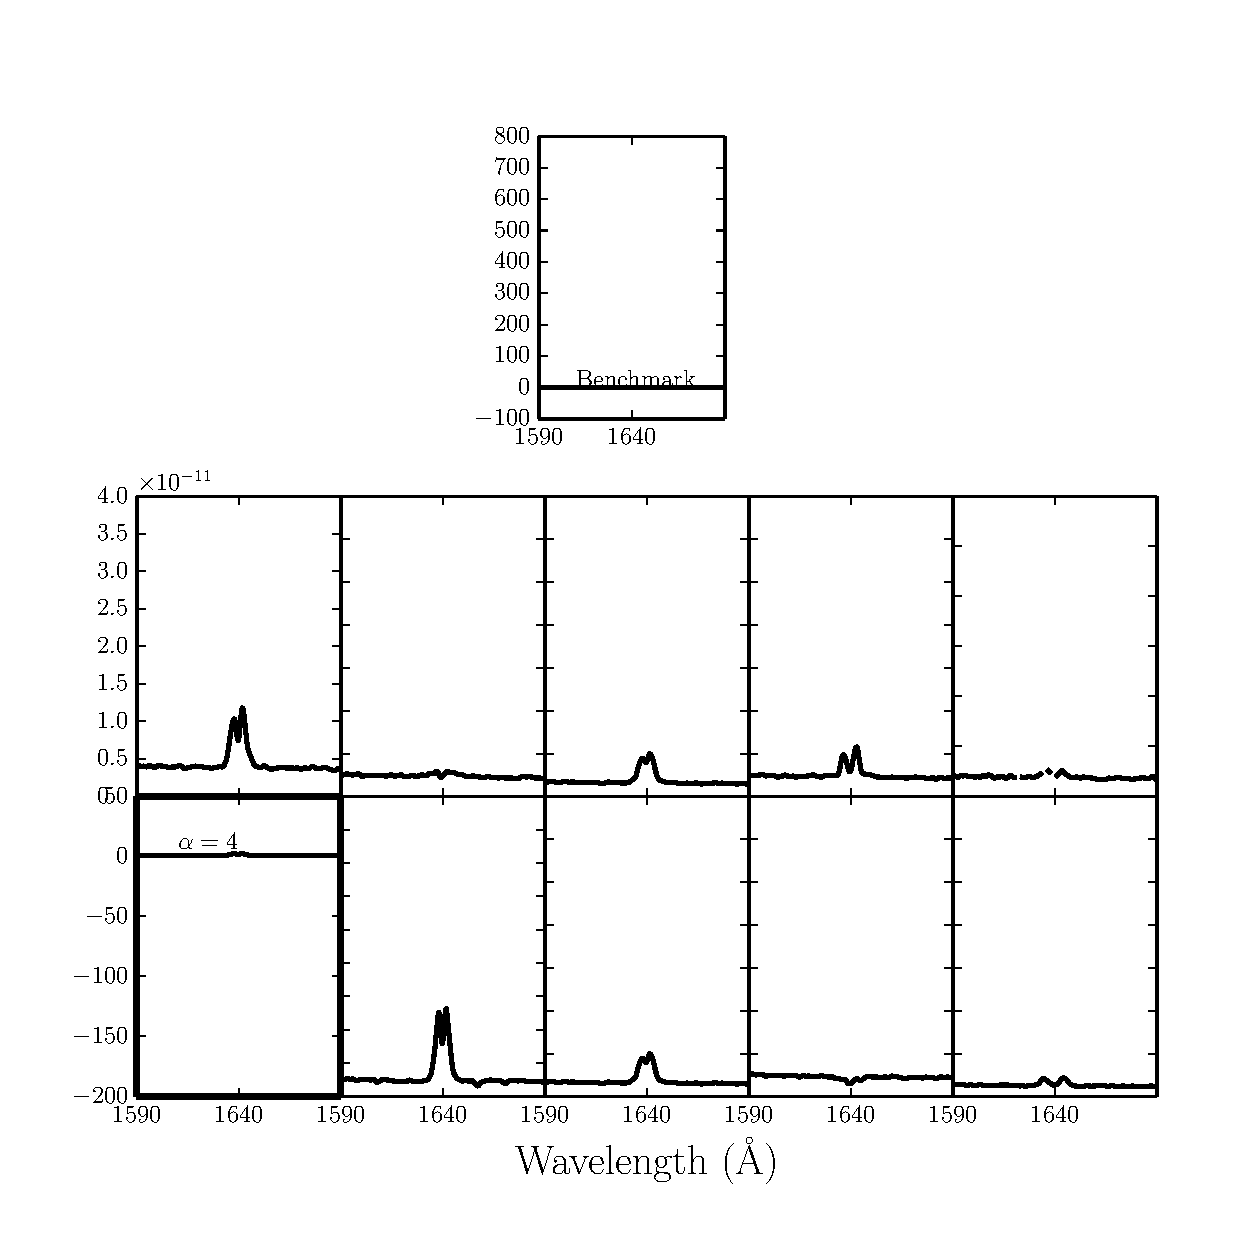
\includegraphics[width=0.5\textwidth]{figures/grid_1640.eps}}
\quad
\subfigure{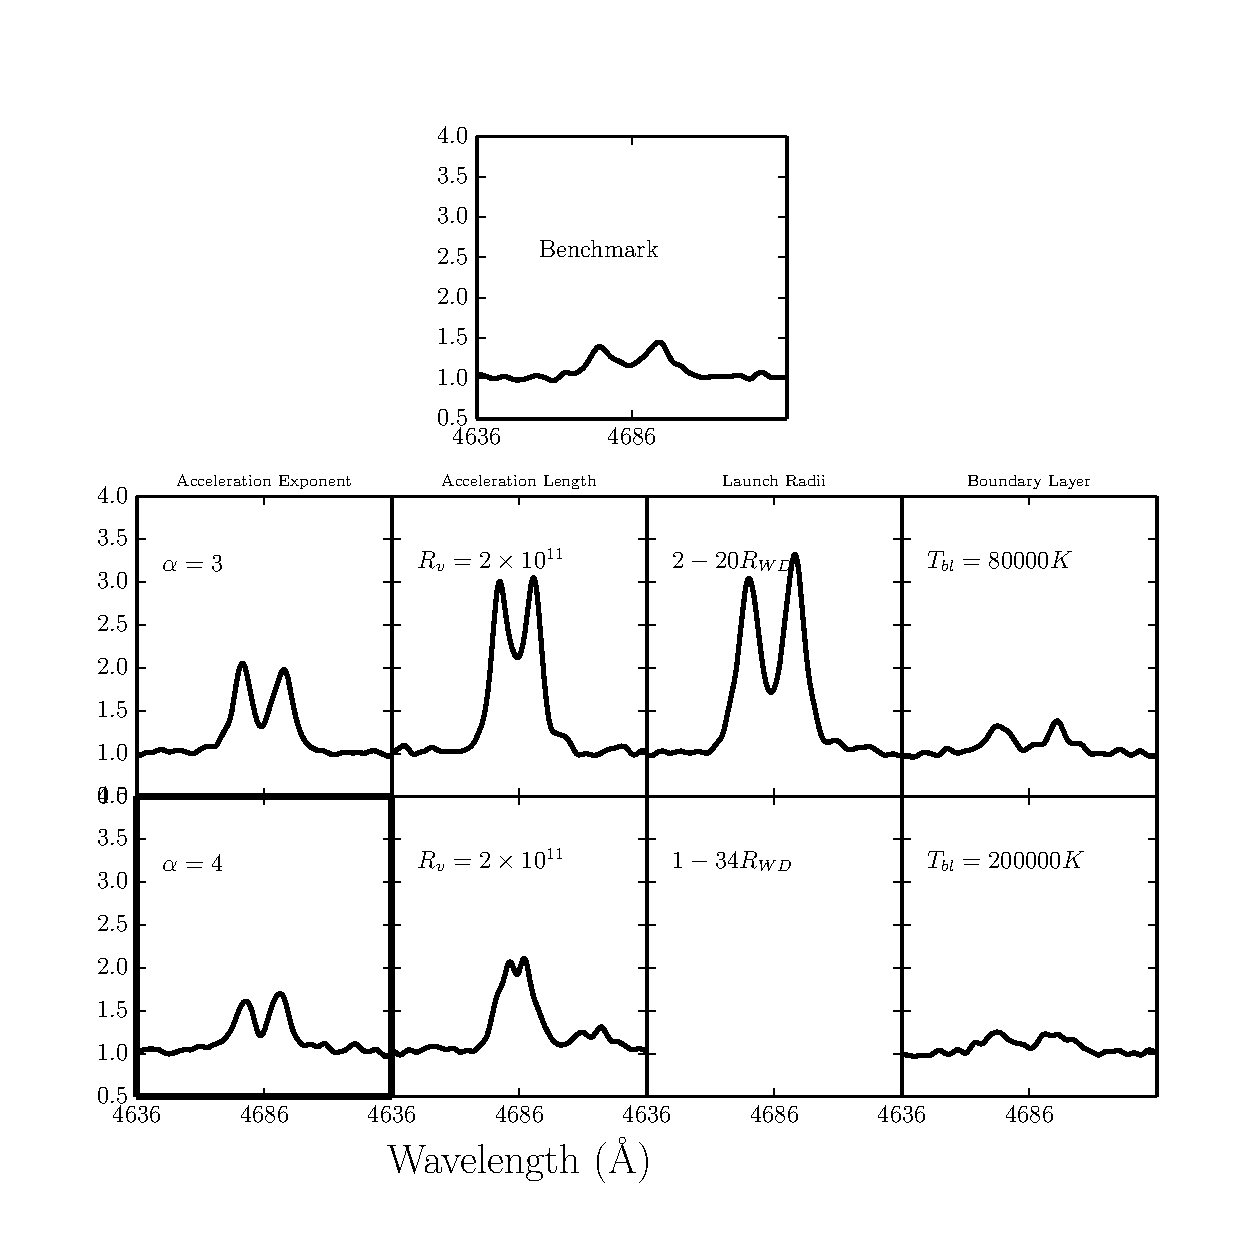
\includegraphics[width=0.5\textwidth]{figures/grid_4686.eps}}   
}
%%\includegraphics[width=0.5\textwidth]{figures/test.eps}
\caption{
The evolution of the He II lines with the kinematic properties
of the wind. 
% The panels are ordered in the same way as figure~\ref{halpha}. In general, increasing densities
% lead to a Balmer jump in emission, although as in the case of H$\alpha$ there is a transition
% when the wind becomes a neutral absorbing column.
}
\label{jump}
\end{figure}



\subsection{Helium Lines}
Discussion of Helium lines in the spectrum.
\begin{itemize}
\item He II 4686, He II 1640 strengths
\item Make the prediction that if 4686 is strong we might expect strong He II 3202. 
\item Discuss why it wouldn't have been seen yet (spectral coverage)
\item Helium I lines
\end{itemize}

\begin{figure} %fullpage
\mbox{
\subfigure{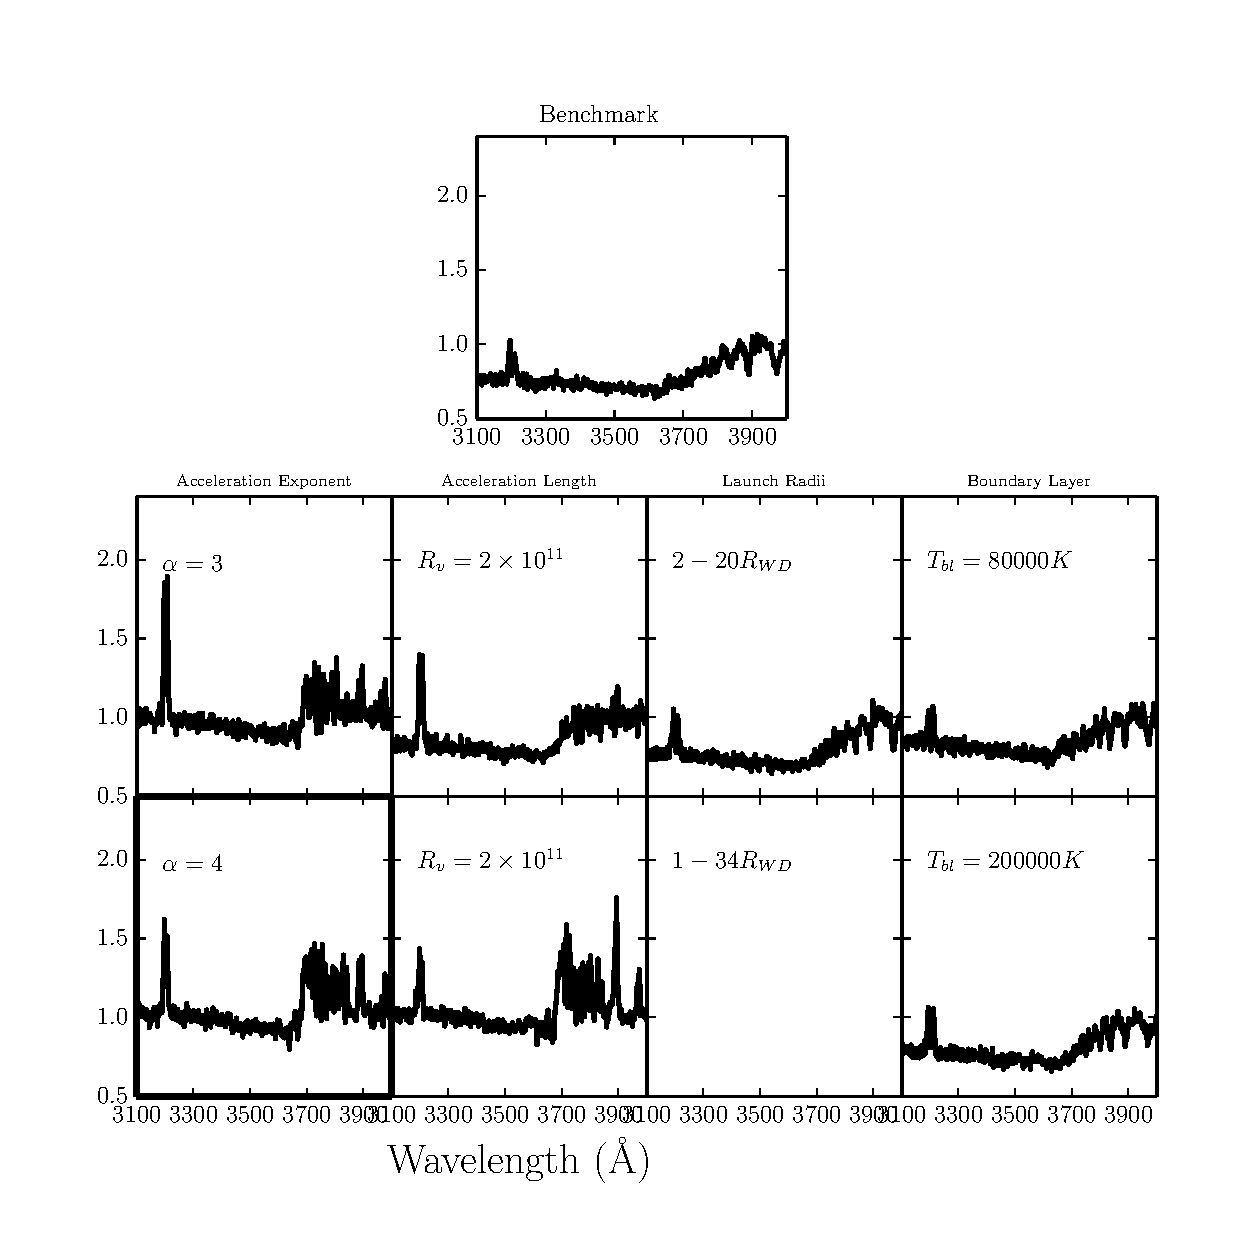
\includegraphics[width=0.5\textwidth]{figures/grid_balmer.eps}}
\quad
\subfigure{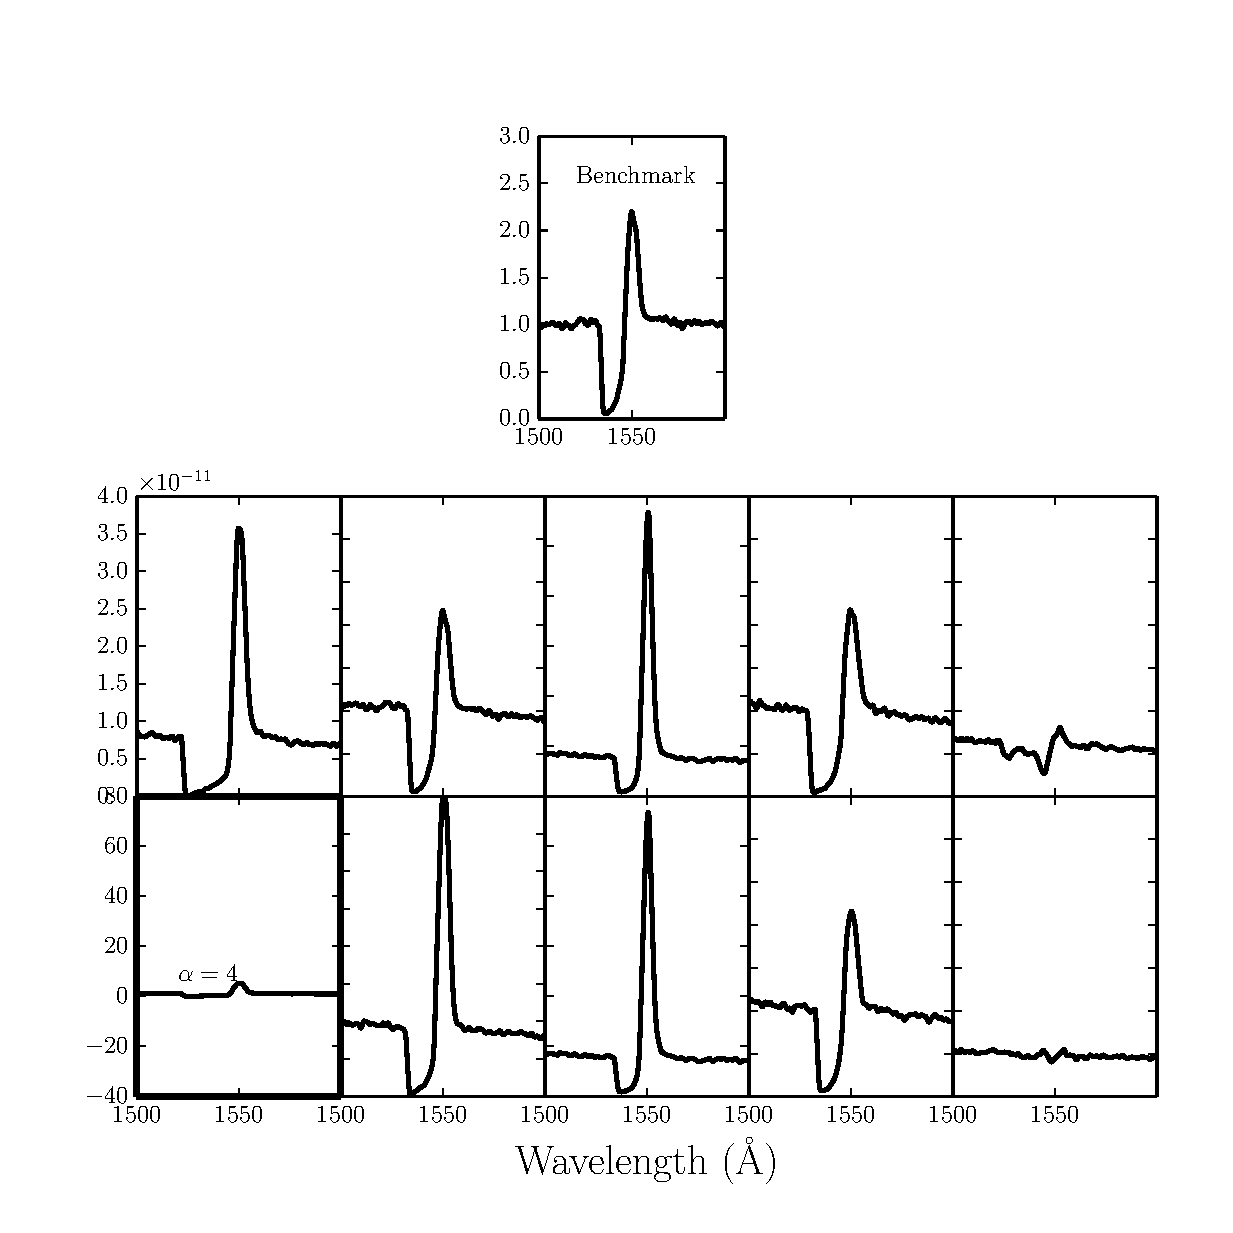
\includegraphics[width=0.5\textwidth]{figures/grid_uv.eps}}   
}
%%\includegraphics[width=0.5\textwidth]{figures/test.eps}
\caption{The evolution of the Balmer jump and C~\textsc{iv} line with the kinematic properties
of the wind. 
% The panels are ordered in the same way as figure~\ref{halpha}. In general, increasing densities
% lead to a Balmer jump in emission, although as in the case of H$\alpha$ there is a transition
% when the wind becomes a neutral absorbing column.
}
\label{jump}
\end{figure}



\subsection{UV Resonance Lines}
Compare spectra to LK02 and other models. Are the spectral features preserved, has anything significant changed.
Lyman alpha?



\subsection{Boundary Layer}
\begin{itemize}
\item discuss the effect of 80000K and 200000K Boundary layers
\item Particularly referring to He II and CIV
\item Our findings support idea that 200000K BL would over ionize the wind- 
we favour 80,000K
\item I'd like to do a hypothetical Zanstra calculation here- state what
temperature our model would predict from the Zanstra method
\end{itemize}

%\subsubsection{The Line Force}
%\begin{itemize}
%\item Can this wind be radiatively driven? 
%\item Why/why not?
%\item Figure showing line force throughout the wind as a fraction of some critical value?
%\end{itemize}


\newpage

%%%%%%%%%%%%%%%%%%%%%%%%%%%%%%%%%%%%%%
%
%          Comparison with real spectra
%
%%%%%%%%%%%%%%%%%%%%%%%%%%%%%%%%%%%%%%%

\section{A Next-Generation Model}

\begin{table}
\centering
\begin{tabular}{p{3cm}p{4cm}}
Model B \\
\hline Free Parameters 	&	 Value \\ 
\hline \hline 
$M_{WD}$ 	 &	 $0.8 M_{\odot}$ \\ 
$\dot{M}_{acc}$ 	 &	 $10^{-9}~M_{\odot}yr^{-1}$\\ 
$\dot{M}_{wind}$  &	$10^{-8}~M_{\odot}yr^{-1}$\\ 
$r_{min}$ 	&	 $4 R_{WD}$\\ 
$r_{max}$ 	&	 $12 R_{WD}$ \\ 
$\theta_{min}$ 	&	 $20.0^{\circ}$ \\ 
$\theta_{max}$ 	&	 $65.0^{\circ}$ \\ 
$\gamma$ 	&	 $1$ \\ 
$v_{\infty}$ 	&	 $3v_{esc}$ \\ 
$R_v$ 	        &	 $1\times10^{11}$cm \\ 
$\alpha$ 	&	 $4$ \\
\end{tabular}
\centering
\caption{Wind geometry parameters used in the next-generation CV model.}
\label{modelb}
\end{table}

With modest changes to the kinematics of the benchmark CV model,
it is possible to produce a `next generation model' with enhanced
line emission that comes closer to reproducing the observed optical spectrum
of a Nova-like variables. The parameters for this model (imaginatively dubbed Model B)
are show in table~\ref{modelb}, and the synthetic spectrum
is shown in figure~\ref{uvoptb}. An in and out of eclipse comparison 
between the synthetic spectrum
at an angle of $80^\circ$ and the high-inclination nova-like RW Tri 
is also shown in figure~\ref{rwtricomp}.

The similarity with the observed spectrum is striking. 
Model B produces strong emission in all the Balmer lines, 
with line to continuum ratios
comparable to those in RW Tri. 
The line to continuum ratio increases during eclipse,
as one expects if the emission is produced in a disk wind, 
thereby mimicking the behaviour of SW Sex stars.
The single-peaked $H\alpha$ line is produced by our models with a 
very similar width to the observed spectrum, although it is perhaps slightly more
`flat-topped' in the synthesized data.

One of the limitations of the model is that, apart 
from in $H\alpha$, the lines are in general double-peaked. 
The lack of high-resolution data in this regard makes detailed analysis difficult,
but it would appear that understanding how single-peaked 
line emission forms and the kinematics and densities required to
modify the line profile is still an open question. 
The major fallback of the next-generation model, however, lies
in the ultraviolet. To get the required emission in the optical lines
and recombination continuum the densities required are very high.
This causes a significant collisionally excited contribution
to the UV lines, meaning that the red wing of the 
resonance species such as C\textsc{iv} no longer matches the
observed profiles. 




\begin{figure} %fullpage
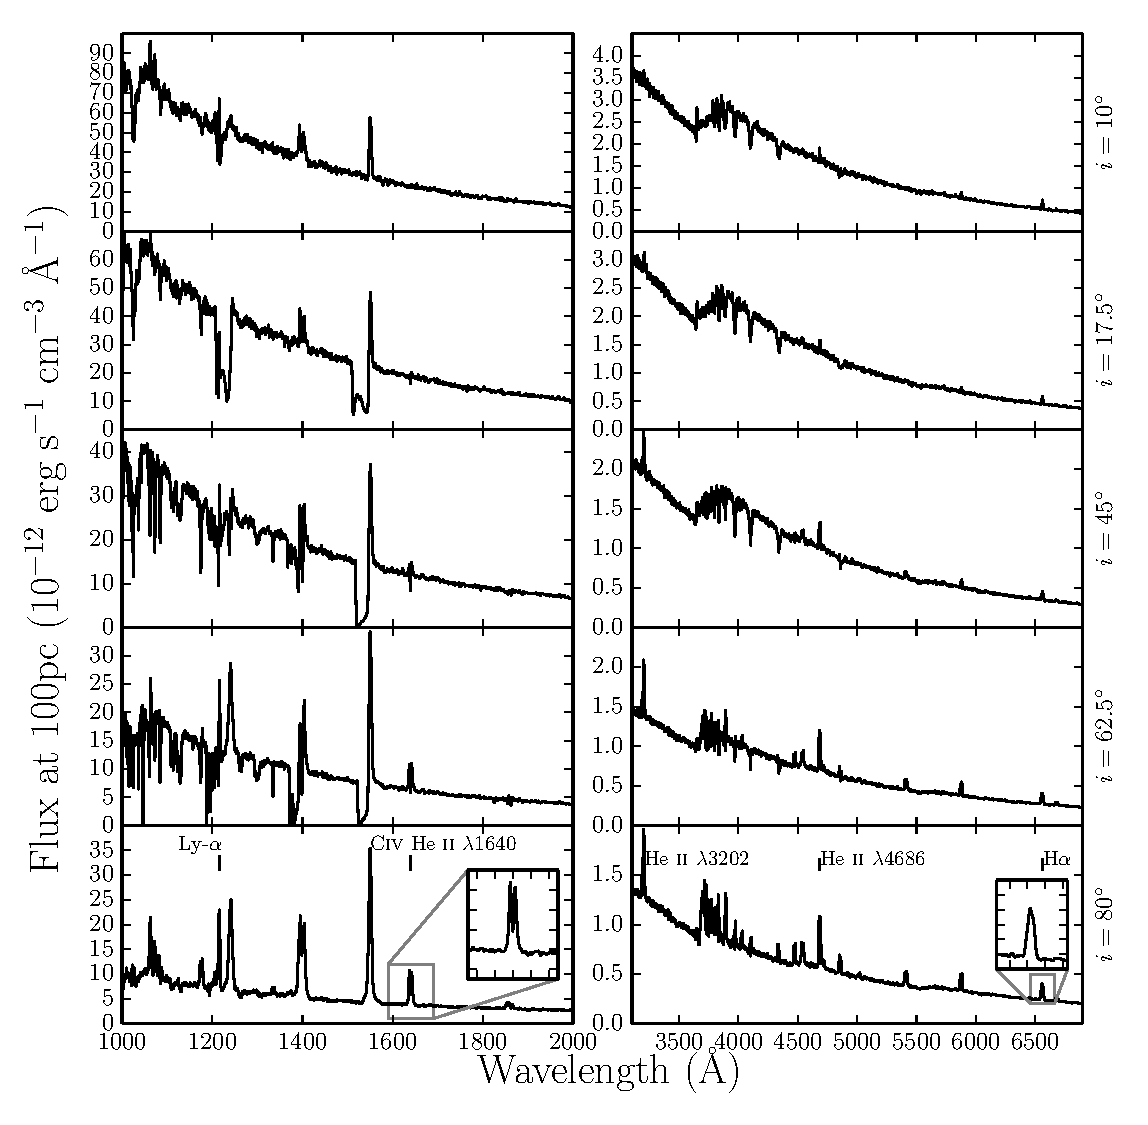
\includegraphics[width=\textwidth]{figures/fig14_uv_opt.eps}
\caption{
UV (left) and Optical synthetic spectra for model B computed at
sightlines of 10,27.5, 45, 62.5 and 80 degrees.	
The inset plots show zoomed-in line profiles for 
\heiiuv and \ha. The \ha line 
is single peaked, but higher order lines in the Balmer series
are double-peaked, albeit with narrower profiles.
Strong \heiiopt emission can be seen
}
\label{uvoptb}
\end{figure} %fullpage


\begin{figure} %fullpage
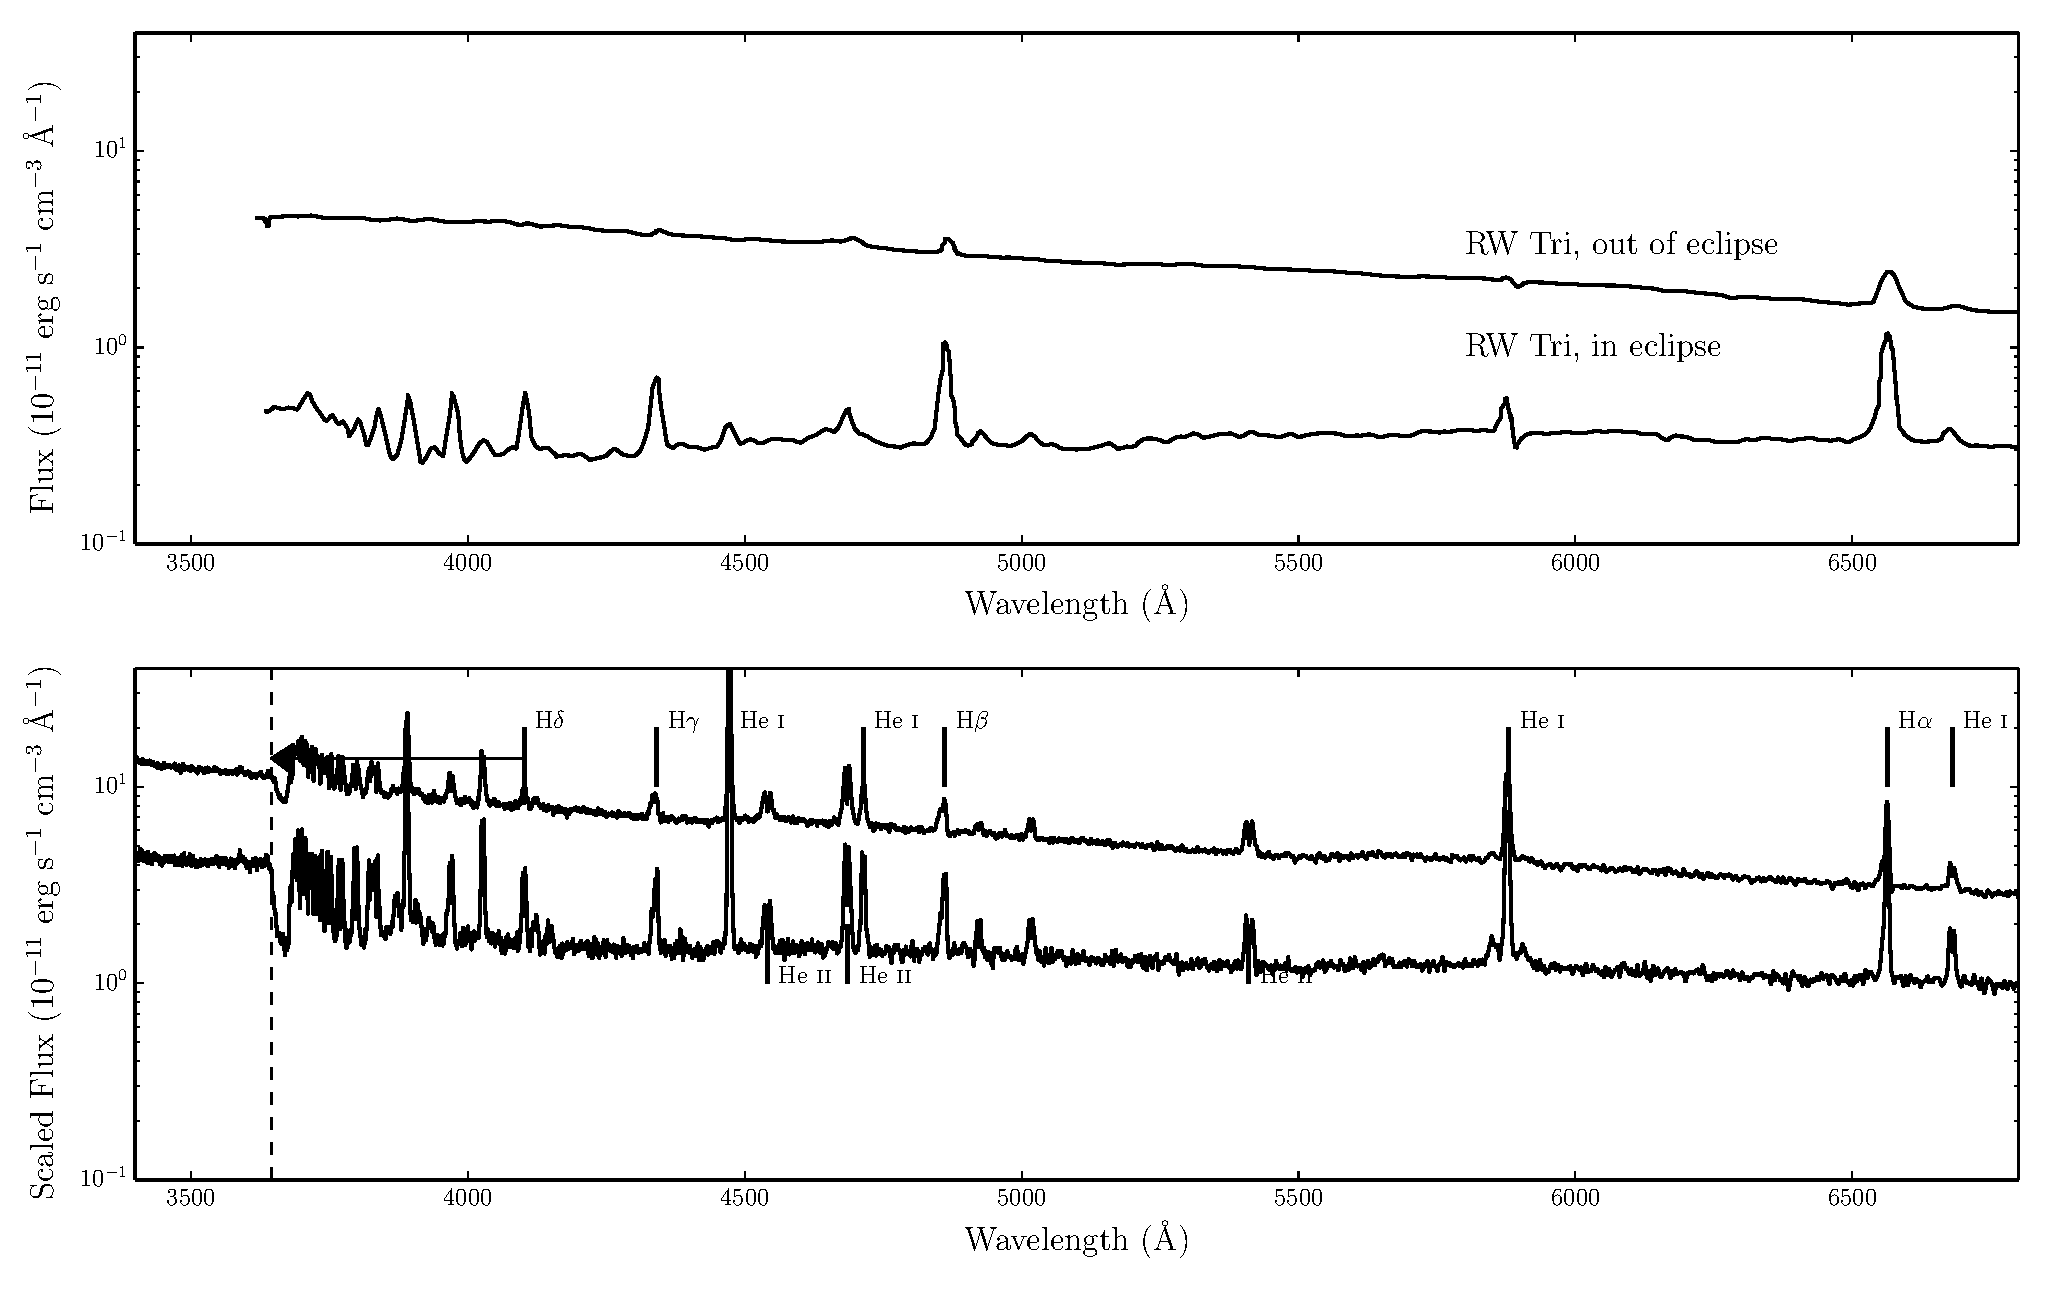
\includegraphics[width=0.8\textwidth]{figures/fig13_eclipse.eps}
\caption{{\sl Top Panel:} In and out of eclipse spectra of the high
inclination Nova-like RW Tri. {\sl Bottom Panel:} In and out of eclipse synthetic
spectra from Model B.}
\label{rwtricomp}
\end{figure} %fullpage




\newpage
%%%%%%%%%%%%%%%%%%%%%%%%%%%%%%%%%%%%%%
%
%          Conclusions and Future Work
%
%%%%%%%%%%%%%%%%%%%%%%%%%%%%%%%%%%%%%%%


\section{Conclusions}

By taking an already successful model
for the UV wavelength regime of CVs and treating 
it with an improved line transfer scheme, we have shown
that the wind does produce some recombination lines
and continuum emission blueward of the Balmer edge.
We have confirmed a number of the expected trends
by exploring a limited number of parameters governing the
kinematics and geometry of the wind. These include:

\renewcommand{\labelitemi}{$\bullet$}
\begin{itemize}
	\item The `filling-in' of the Balmer jump \citep{elitzur1983} by recombination 
	continuum emission from a disk wind
	\item Single peaked line emission in H alpha produced by 
	the introduction of a poloidal velocity gradient \citep{MC96}
	\item A Balmer decrement consistent with optically thick emission \citep{elitzur1983}.
\end{itemize}
\smallskip

\noindent We also make a number of predictions:

\begin{itemize}
	\item The depth of the Balmer absorption edge decreases with increasing inclination,
or alternatively that the Balmer recombination emission
is enhanced at higher inclinations, {\sl relative to the disk continuum}.
	\item The He~\textsc{ii}~$\lambda3202{\rm \AA}$ line should be
prominent in cases where He~\textsc{ii}~$\lambda1640{\rm \AA}$ \& 
\heiiopt are seen. 
	\item A Balmer jump in emission during eclipse.
\end{itemize}

\smallskip
We have presented a next-generation model
which produces all the prominent lines in and out of eclipse, and
shown that the model exhibits verisimilitude with the optical spectrum of RW Tri.
However, this model does not produce a complete unified CV model, as
the emission lines in the UV are somewhat unrealistic in strength.
This is a shortcoming which must be understood if it is true that
disk winds modify line profiles to become single peaked, as the 
densities required produce a large amount of collisionally excited emission
in UV resonance lines.

Our work demonstrates that, if nothing else,
{\sl disk winds matter}. At a minimum,
they can act as a spectral filter
for the disk spectrum. At a maximum, they may be responsible
for the majority of spectral features of high-state CVs,
and could dominate the appearance of both UV and optical
spectra of these systems.

%% Balmer jump


% \subsection{Future Work}

% To further investigate the true effect of the wind
% we hope that high quality, broadband spectra of 
% Nova-like variables at a range of inclinations 
% will be taken to examine 

% In addition to this project, we have started to apply the macro atom scheme to QSOs in order to build on the work of Higginbottom et al. (2013). In particular, we hope that the macro-atom scheme will enable the
% model to produce significant Lyman-$\alpha$ emission, as is observed in QSOs.


\subsection*{Acknowledgements}
The work of JHM, NH and CK is supported by the Science and Technology Facilities Council (STFC), 
via studentships and a consolidated grant, respectively. We would like to thank Juan Hernandez Santisteban and Ivan Hubeny 
for useful discussions. We acknowledge the use of the IRIDIS High Performance Computing Facility, 
and associated support services at the University of Southampton, in the completion of this work.


\newpage
\newpage
\bibliography{mybib.bib}

\end{document}
